

\definecolor{listinggray}{gray}{0.9}
\definecolor{lbcolor}{rgb}{0.9,0.9,0.9}
\lstset{
	backgroundcolor=\color{lbcolor},
	tabsize=4,
	rulecolor=,
	language=matlab,
        basicstyle=\scriptsize,
        upquote=true,
        aboveskip={1.5\baselineskip},
        columns=fixed,
        showstringspaces=false,
        extendedchars=true,
        breaklines=true,
        prebreak = \raisebox{0ex}[0ex][0ex]{
          \ensuremath{\hookleftarrow}},
        frame=single,
        showtabs=false,
        showspaces=false,
        showstringspaces=false,
        identifierstyle=\ttfamily,
        keywordstyle=\color[rgb]{0,0,1},
        commentstyle=\color[rgb]{0.133,0.545,0.133},
        stringstyle=\color[rgb]{0.627,0.126,0.1},
}
\newcommand{\avg}[1]{\langle #1 \rangle}

\chapter{Implementation of a robust structured illumination
  reconstruction technique}

\section{On the numerical test sample}


As a test object I create a sphere shell, a line and a rectangle.
That is shown in the following code.  The objective is a NA1.4 oil
with coherent \unit[473]{nm} excitation light and detection is at
\unit[520]{nm} (incoherent).

The following listing shows how the image of the grating for
non-uniform excitation is calculated. The z-section of the result is
shown in \figref{fig:grating}. The illumination source is coherent
therefore the grating structure is visible over quite a large
z-distance (due to the reimaging by the Talbot effect).


\begin{lstlisting}
n=128;
nmperpixel=100;
sz=2;
NA=1.4;
znmperpixel=sz*nmperpixel;
%% vector psf for excitation illumination
asf=squeeze(kSimPSF({'lambdaEx',473;'na',NA;'ri',1.518;...
    'sX',n;'sY',n;'sZ',sz*n;...
    'scaleX',nmperpixel;'scaleY',nmperpixel;'scaleZ',znmperpixel;...
    'computeASF',1}));


%% grating of period P
% one pixel is 100nm so the period is P*100nm
P=6;
grat2d=(mod(xx(n,n),P)>(floor(P/2)-1))*1000;
%% fill a 3d grating
grat=newim(n,n,sz*n);
grat(:,:,(sz*n)/2)=grat2d(:,:);
kgrat=ft(grat);

%% coherent imaging
imgratx=ift(kgrat.*ft(squeeze(asf(:,:,:,0))));
imgraty=ift(kgrat.*ft(squeeze(asf(:,:,:,1))));
imgratz=ift(kgrat.*ft(squeeze(asf(:,:,:,2))));
imgrat=abs(imgratx).^2+abs(imgraty).^2+abs(imgratz).^2
\end{lstlisting}

\begin{figure}[htb]
  \centering
  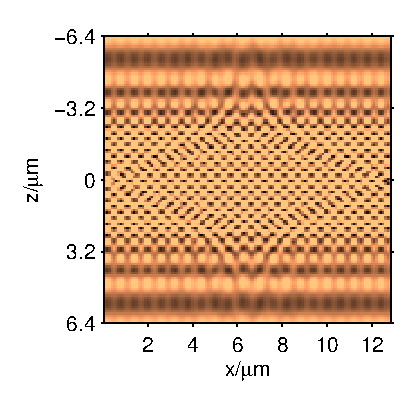
\includegraphics{../app_hilo/grating_xz}

  \caption{x-z-Section {\tt imgrat(:,64,:)} of the coherent
    image of the grating in object space.}
  \label{fig:grating}
\end{figure}

The following listing shows how the sample object (i.e. fluorophore
concentration) is generated.  It consists of a spherical shell
(calculated by the product of two Sinc functions in k-space and a
product with $r$ in real space). There is also a vertical line and a
rectangle. A slice through the simulated fluorophore concentration is
shown \figref{fig:input} left.

The shift by {\tt dz} in z-direction is done by multiplication with
$\exp(-ik{\tt dz})$ in k-space. This is only a good method to defocus
small distances {\tt dz} as the object will wrap around the borders.

\begin{lstlisting}
%% as an object I want a hollow sphere
% I define it in k-space
kobj=sinc(rr(kpsf)./2).*sinc(rr(kpsf)./0.7);

% this is the sphere
obj=rr(psf).*abs(ift(kobj));
maximum=max(obj);
% in-focus rectangle in right top
obj(83:114,23:43,(sz*n)/2)=4*maximum;
% in-focus line on the left
obj(21:21,40:90,(sz*n)/2)=12*maximum;

%% shift the object a little bit in z
kobj=ft(obj);
dz=1; % shift in pixels -> 1 equals 100nm
kobj=kobj.*exp(-i*2*pi*zz(kobj,'freq')*dz);
obj=ift(kobj);
\end{lstlisting}

In order to simulate the final image the fluorophore concentration is
multiplied by the excitation field and the result is convolved with
the PSF of the microobjective (this time according to the rules of
incoherent imaging). The Matlab code for this is shown in the
following listing:
\begin{lstlisting}
%% for imaging the fluorescence light
psf=kSimPSF({'lambdaEx',473;'lambdaEm',520;'na',1.4;'ri',1.518;...
        'sX',n;'sY',n;'sZ',sz*n;...
        'scaleX',nmperpixel;'scaleY',nmperpixel;'scaleZ',znmperpixel});
%% ft thereof
kpsf=ft(psf);
%% excited fluorophores
fluo=obj.*imgrat;

%% fluorescence image with structured illumination
strucflimg=ift(ft(fluo).*kpsf);

%% widefield fluorescence image
flimg=ift(ft(obj).*kpsf);

%% extract focal planes
iu=real(squeeze(flimg(:,:,(sz*n)/2)));     % uniform illumination
in=real(squeeze(strucflimg(:,:,(sz*n)/2)));% structured illumination
\end{lstlisting}


The image for uniform illumination is shown in
the middle of \figref{fig:input}. The right picture shows the image
for non-uniform illumination with the \unit[600]{nm}-period grid.

\begin{figure}[htb]
  \centering
  \subfigure[object]{
\includegraphics[width=4cm]{../app_hilo/obj}}
  \subfigure[widefield illumination]{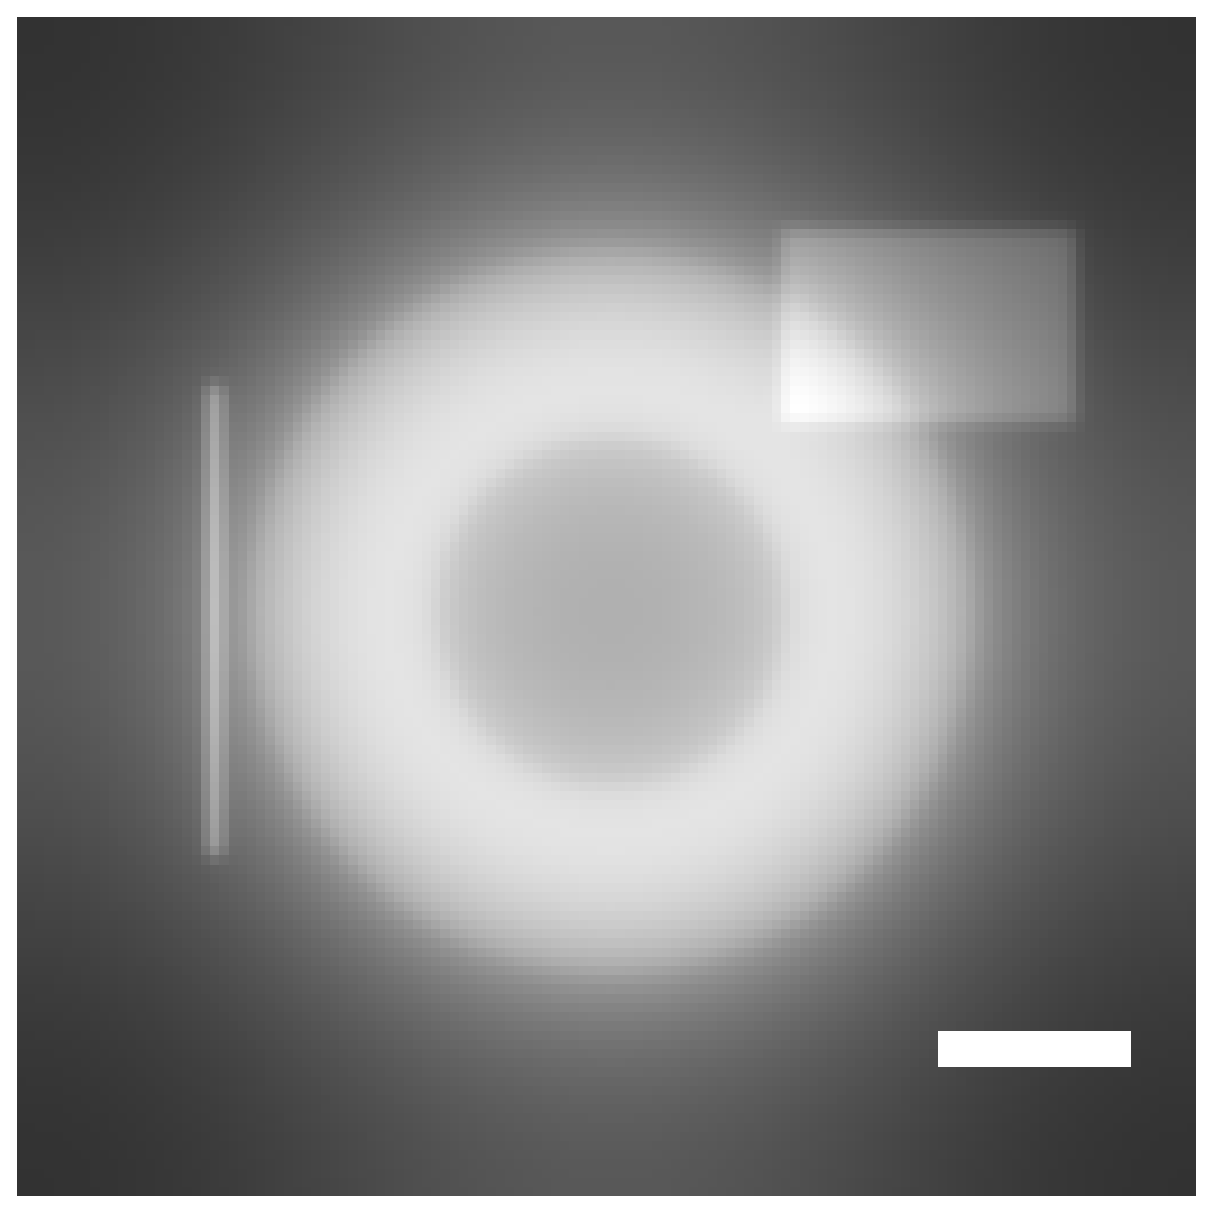
\includegraphics[width=4cm]{../app_hilo/iu}}
  \subfigure[structured illumination]{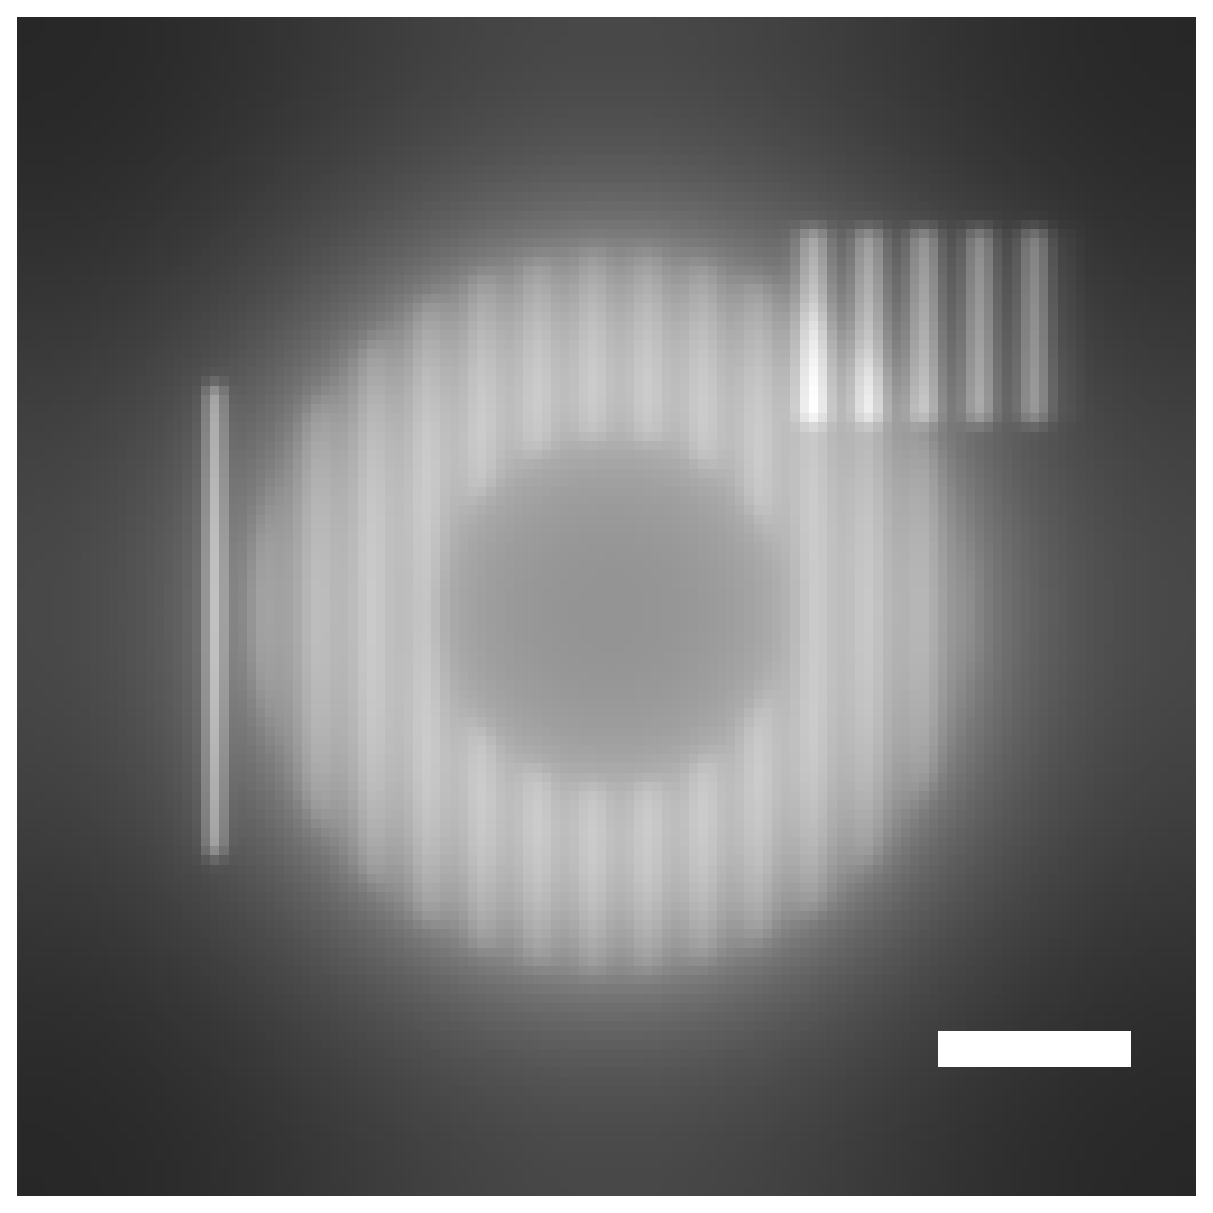
\includegraphics[width=4cm]{../app_hilo/in}}
  \caption{Slice of the object in the focal plane. It consists of a
    line, a spherical shell and a rectangle. Only the shell is
    extended in z. {\bf(a)}, Image with widefield
    illumination. {\bf(b)}, Image with structured illumination
    (grating period \unit[600]{nm}). {\bf(c)} The scalebar is
    \unit[2]{$\mu$m} wide. }
  \label{fig:input}
\end{figure}

\figref{fig:defocus} shows the non-uniformly illuminated images for
the object being moved relative to the plane of focus. The line and
the rectangle are both blurred and the contrast of the grating
decreases.
\begin{figure}[htb]
  \centering
  \subfigure[100 nm defocus]{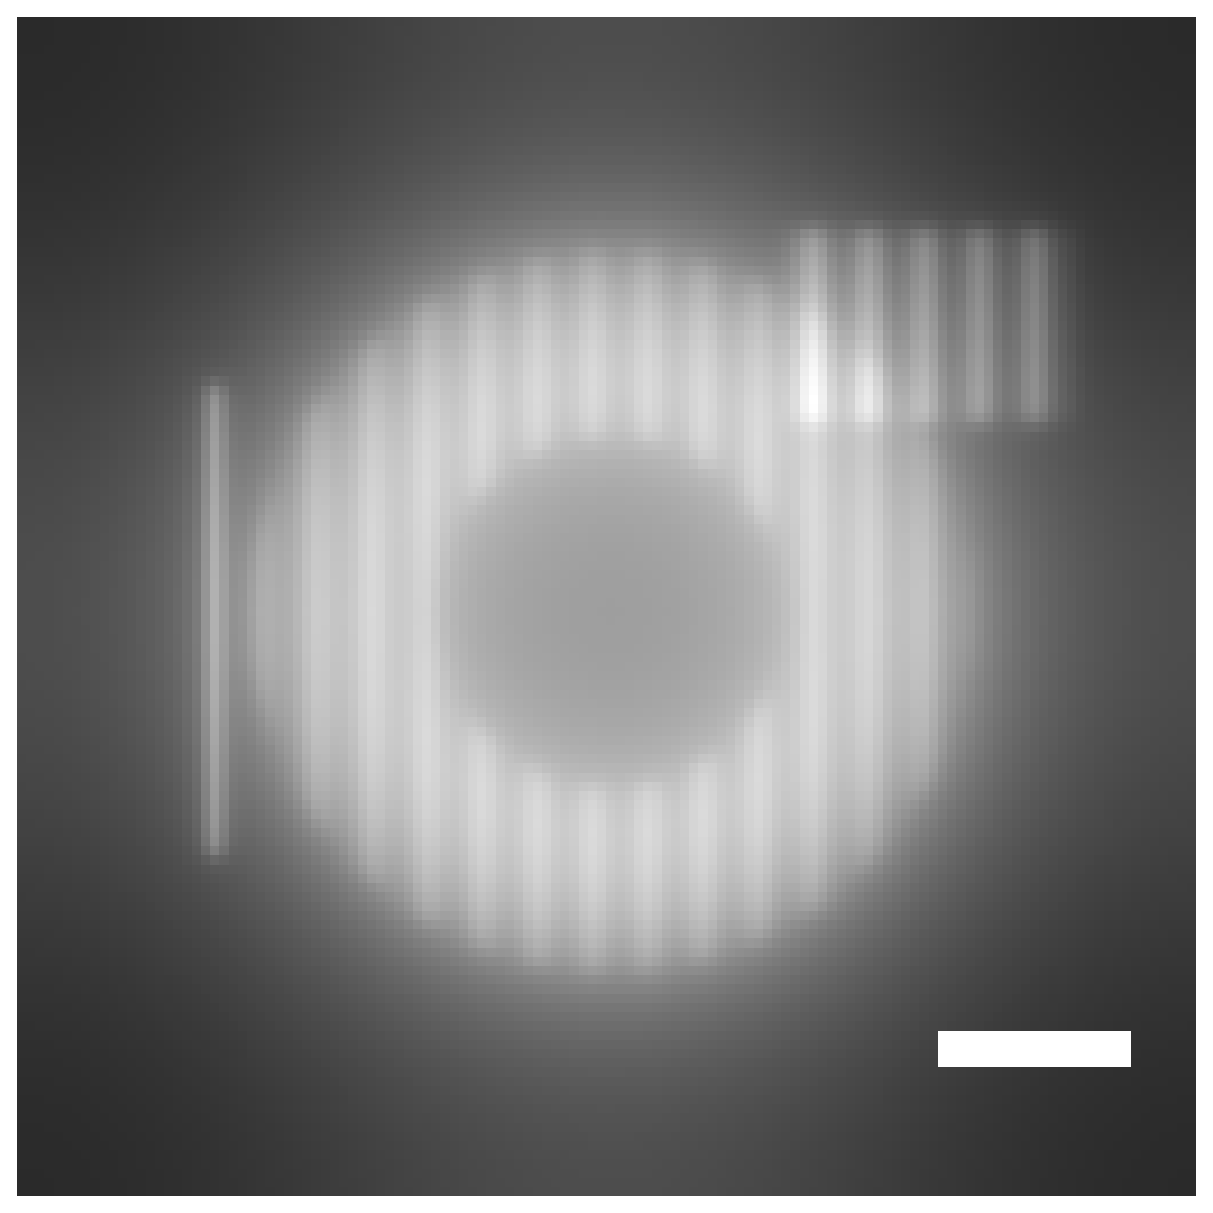
\includegraphics[width=4cm]{../app_hilo/in100}}
  \subfigure[200 nm]{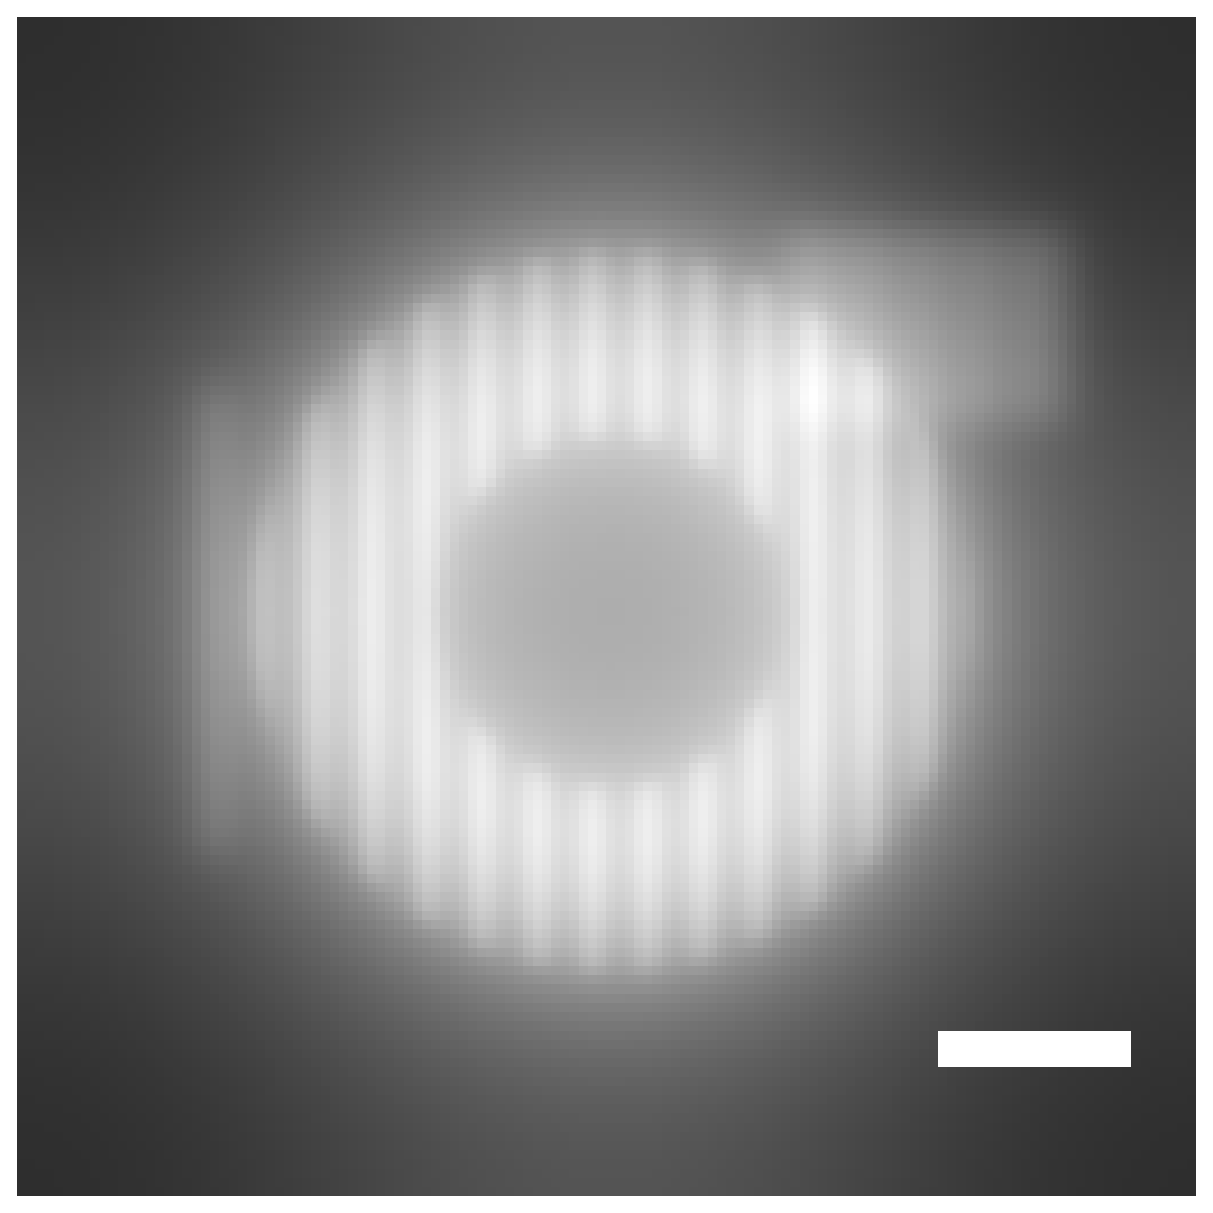
\includegraphics[width=4cm]{../app_hilo/in200}}
  \subfigure[500 nm]{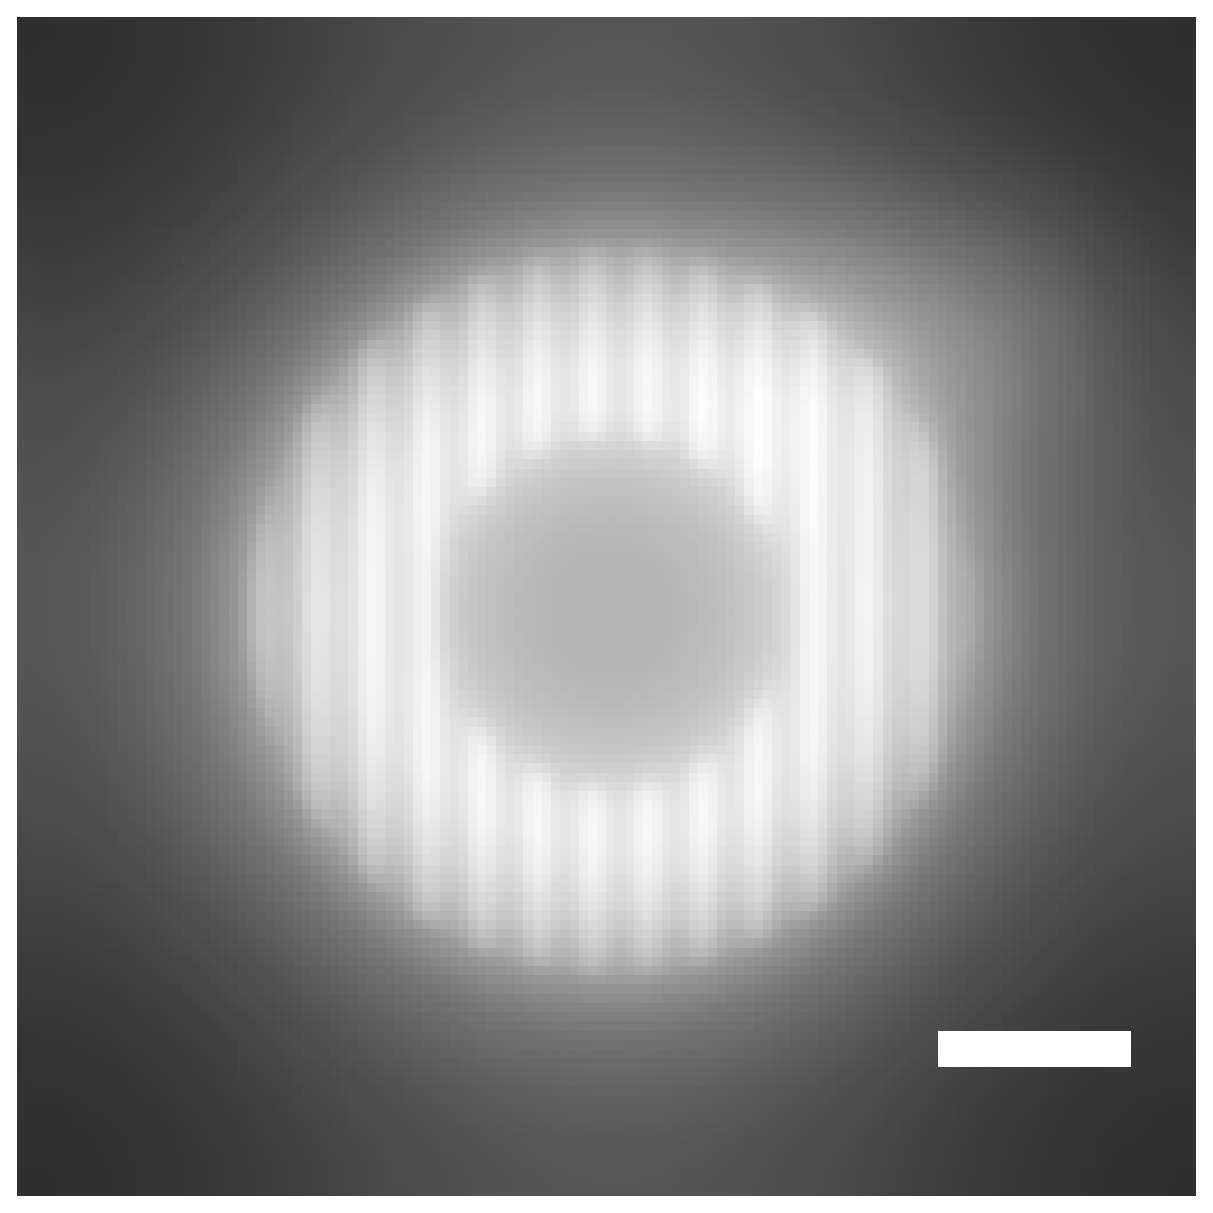
\includegraphics[width=4cm]{../app_hilo/in500}}
  \caption{Defocus series of the test object under structured coherent
    illumination (grating period \unit[600]{nm}). The scalebar is
    \unit[2]{$\mu$m} wide.}
  \label{fig:defocus}
\end{figure}


\section{State of the Art}
If a fluorescent plane is imaged with a fluorescence widefield
microscope, the intensity of the image is constant no matter if the
plane is in-focus or not. 
\subsection{Apotome}
Using non-uniform excitation light the Wilson group was able to
circumvent this problem (\cite{1997Neil}). They project a grid pattern
into the sample. For a fluorescent plane sample the modulation in the
image is highest, when the sample is in-focus. If the plane is moved
out of focus, the modulation decreases. Hence it is possible to achieve
z-sectioning in a widefield microscope.

For one section $I_p$ they combine three grating images $I_i$ (grating
period $1/\nu$) with different phases:
\begin{align}
  I_p=\abs{I_1+I_2e^{i2\pi/3}+I_3e^{i4\pi/3}}
  \sim\abs{ 2 \frac{J_1(2u\nu(1-\nu/2))}{u\nu(1-\nu/2)}}.
\end{align}

The last term is their result for the intensity of a fluorescent plane
with the defocus $u$. If no grating is displayed ($\nu=0$) the
resulting image $I_p$ is constant and the microscope has no sectioning
capability. A fine grating gives best sectioning capability (but one
has to make a tradeoff as a fine grating will give very low contrast
in a thick specimen).

For this method is necessary to capture three images to generate one
sectioned slice. This can be a problem if the movement of the grating
isn't perfect or if the object moves during these exposures.

\subsection{HiLo}
This problem is addressed by Jerome Mertz et al.\ (\cite{2008Lim},
\cite{2009Santos}). They discovered that only two images need to be
captured for each z-sectioned slice.
An image with uniform illumination contains contributions
of both in-focus and out-of-focus fluorophores:
\begin{align}
\label{eqn:Iu}
  I_u(x,y)=I_\textrm{in}(x,y)+I_\textrm{out}(x,y).
\end{align}
Due to the structure of the OTF out-of-focus light is limited to low
spatial frequencies.

The modulated part of the non-uniformly illuminated image contains only
information of the in-focus object structure:
\begin{align}
\label{eqn:In}
  I_n(x,y)&=I_\textrm{in}(x,y)(1+M
  \sin(\kappa x+\varphi))+I_\textrm{out}(x,y),\\
  \kappa&=\frac{2\pi}{\lambda}n\sin(\alpha)\nu.
\end{align}

The sectioned image is a combination of high-frequency components of
the widefield image $I_u$ and the low-frequency components of the
modulated part of the non-uniform image $I_n$.


\subsubsection{Speckle}
In the older publication (\cite{2008Lim}) a random speckle pattern is
projected into the sample (presumably because this is experimentally
easier than projecting a grating). For completeness I describe my
reimplementation of their method. 

In order to process the non-uniform image it is divided into
subregions.  As a measure of local contrast in each of these
subregions the relative standard deviation is calculated 
(the operator $\avg{\cdot}$ indicates averaging):
\begin{align}
  c_n=\frac{\sqrt{\avg{I_n^2}-\avg{I_n}^2}}{\avg{I_n}}.
\end{align}
The relative standard deviation $c_n$ will be zero for image regions
without in-focus contributions. Its value increases as the modulation
of the non-uniform illumination increases (that's what we
want). However $c_n$ also increases if there is a small in-focus
feature. In that we are not interested as we only want to build up an
image of in-focus fluorophores with low spatial frequencies. To
correct for that we refer to the most complicated part of the paper
(in my opinion) -- its equation (4). I will repeat their argument
here.

Let $O$ be the image intensity obtained with perfectly uniform
illumination and $S$ the image intensity for the non-uniform
illumination a uniform object. Then the uniformly illuminated image of
the object is:
%FIXME Obviously I still don't understand it!
\begin{align}
  I_u\approx (\avg{O}+\delta O)\avg{S}.
\end{align}
Here the change of $I_u$ due to some object variations $\delta O$ can
only come from in-focus contributions.

\begin{align}
\label{in}
  I_n\approx (\avg{O}+\delta O)(\avg{S}+\delta S).
\end{align}
Here too, $\delta O$ and $\delta S$ come from the focus plane.

The authors state that a corrected relative standard deviation
of the non-uniform illumination can be calculated like this:
\begin{align} 
  c_s^2=\frac{c_n^2-c_0^2}{1+c_0^2}
  =
  \frac{\avg{I_n^2}}{\avg{I_n}^2}
  \frac{\avg{I_u^2}}{\avg{I_u}^2}-1.
\end{align}
Where $c_0$ is the relative standard deviation of the widefield image
$I_u$. The product $I_{su}=c_s\avg{I_u}$ then provides a low
resolution version of $I_u$ that is optically sectioned even for dc
frequencies.

The following listing shows how this algorithm can be applied to two
square input images {\tt iu} and {\tt in}. Instead of doing a discrete
integration over regions I multiply with a gaussian in Fourier
space. The cutoff frequency $k_c$ of the filter is chosen low enough
so that $c_s$ doesn't contain any structure of the grating anymore.
\begin{lstlisting}
si=size(in);
n=si(1);
kc=0.04;
r=rr(in,'freq');
klp=exp(-r.^2/(2*kc^2));
khp=1-klp;
ina=ift(ft(in).*klp);
in2a=ift(ft(in.^2).*klp);
iua=ift(ft(iu).*klp);
iu2a=ift(ft(iu.^2).*klp);
cs2=in2a.*iua.^2./(ina.^2.*iu2a)-1;
isu=sqrt(cs2).*iua;
kihp=ft(iu).*khp;
kilp=ft(isu).*klp;
\end{lstlisting}

\begin{figure}[htb]
  \centering
  \subfigure[Corrected relative standard deviation $c_s$.]{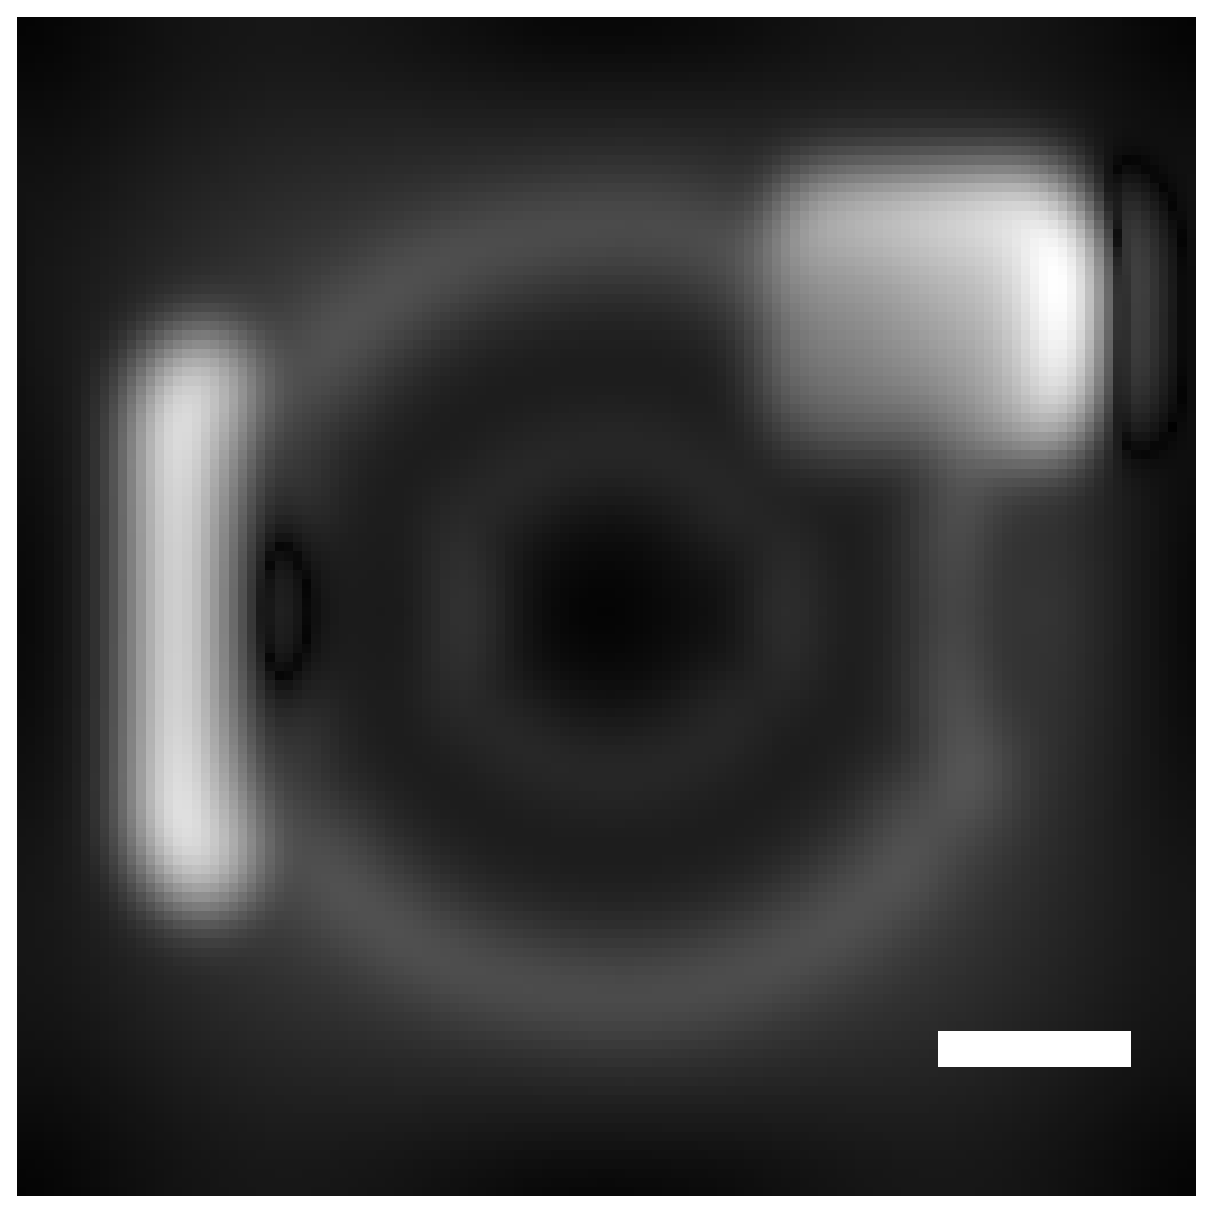
\includegraphics[width=4cm]{../app_hilo/cs}}
  \subfigure[The product $I_{su}=c_sI_u$]{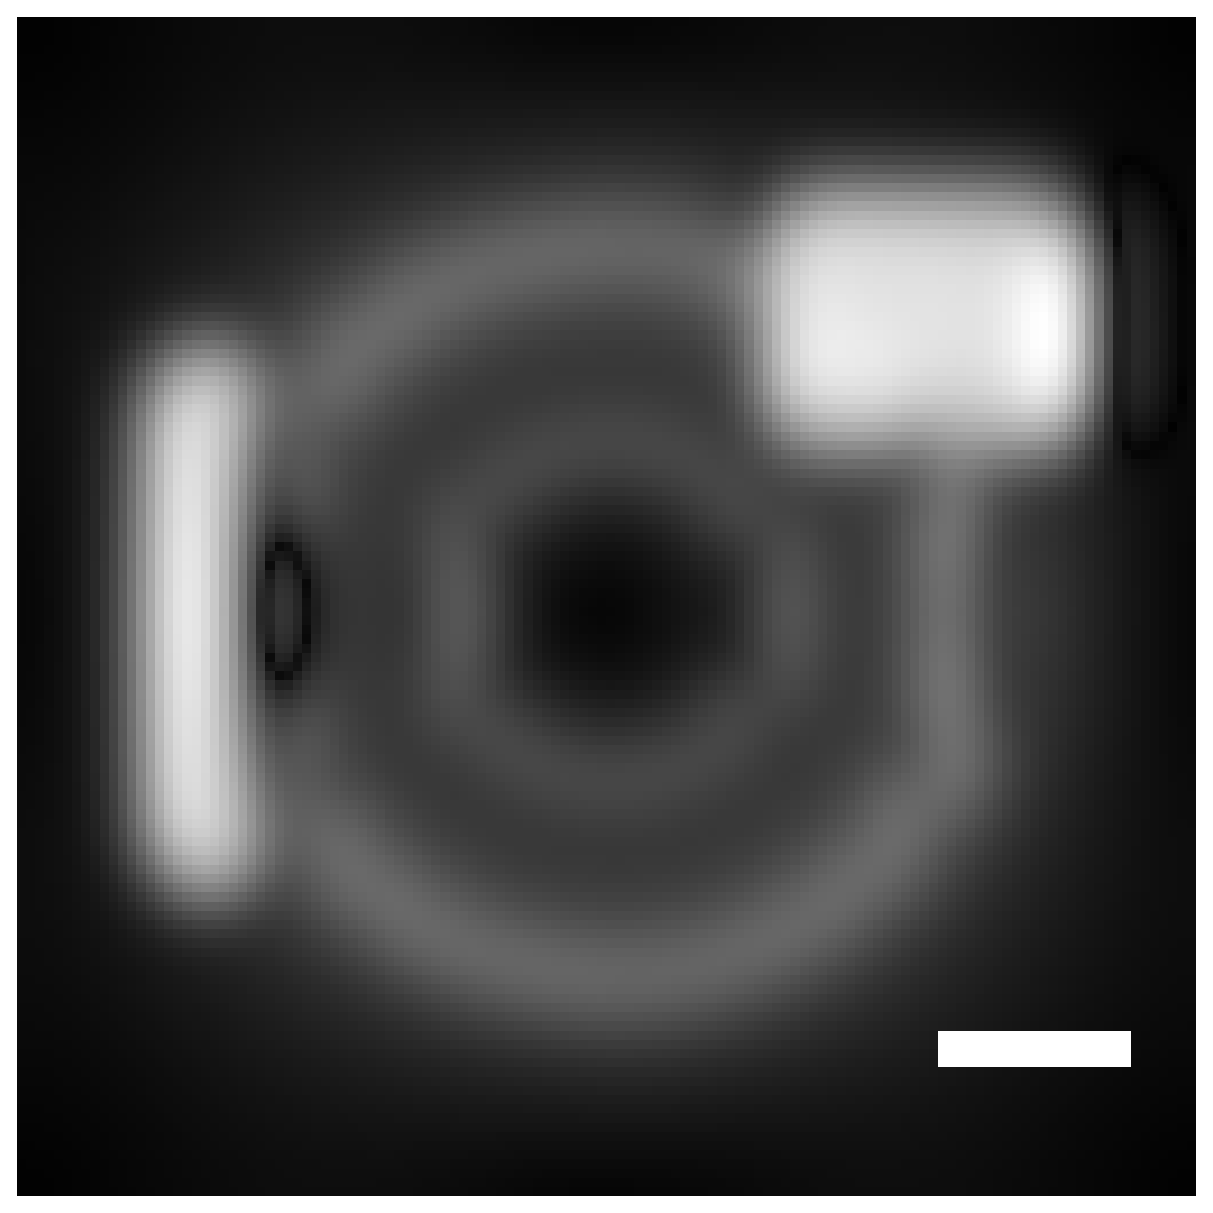
\includegraphics[width=4cm]{../app_hilo/isu}}
  \subfigure[Low spatial frequency section $I_\textrm{lp}$]{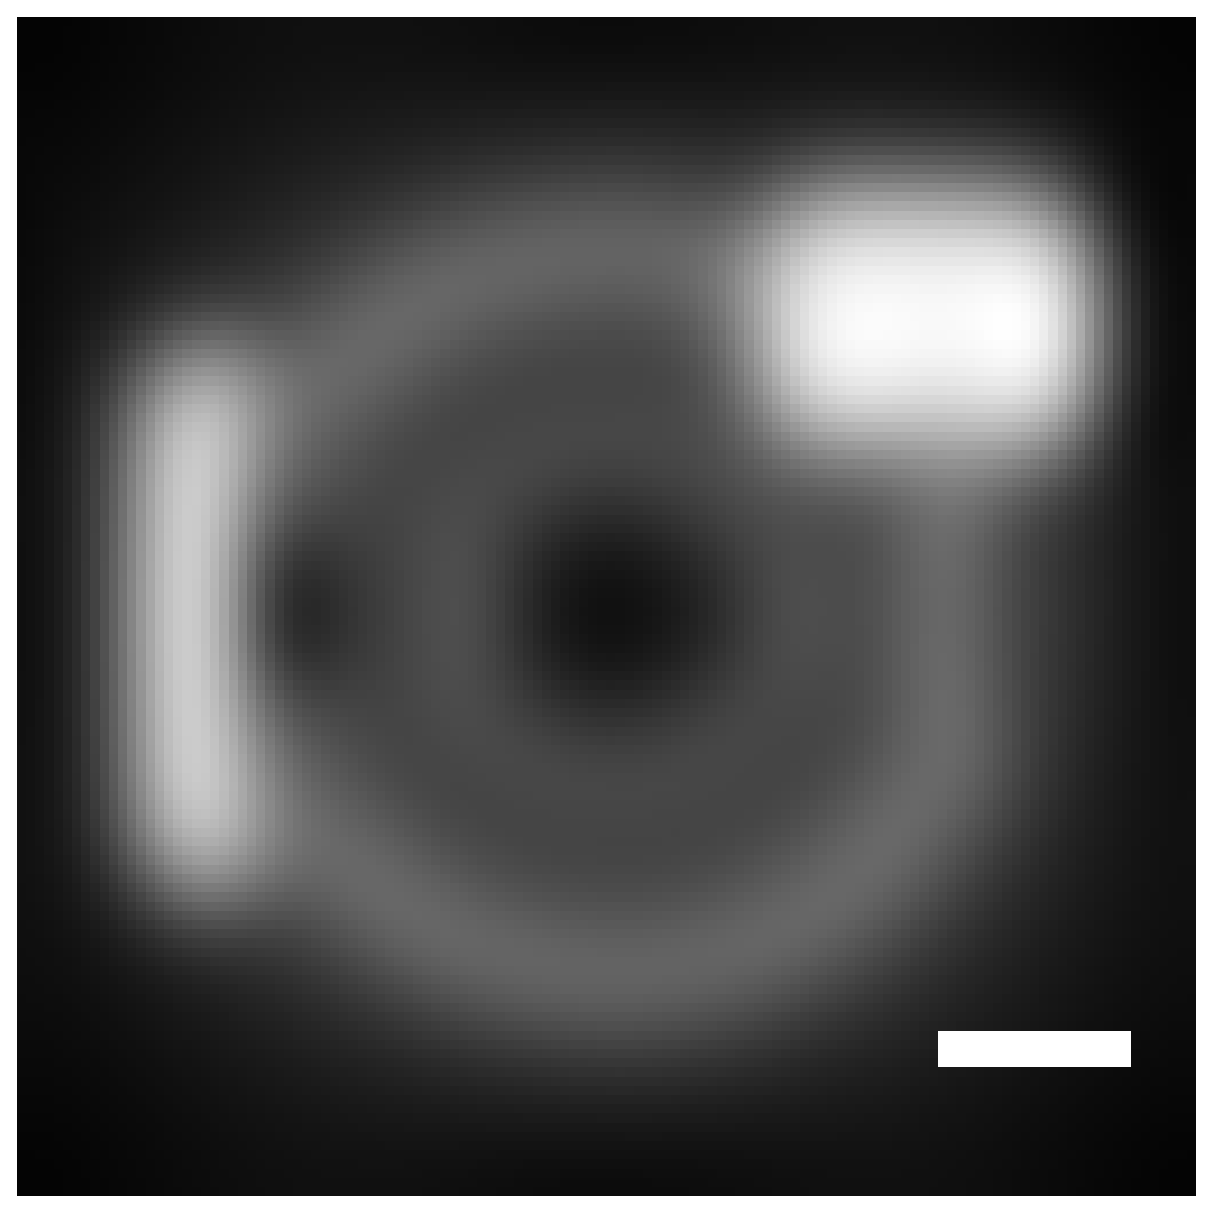
\includegraphics[width=4cm]{../app_hilo/ilp}}
  \caption{Several intermediate results of the algorithm. The scalebar is
    \unit[2]{$\mu$m} wide.}
  \label{fig:hilo1interm}
\end{figure}


The HiLo method combines a low-pass filtered version of $I_{su}$ with
a high pass filtered version of the uniformly illuminated image $I_u$.
To do this the two images are scaled for a seamless interface along
the circle $K$ with radius $\abs{\vect k_c}$ in k-space and then added:
\begin{align}
  \eta=\!\!\!\!\ointop_{\partial K_{k_c}}\!\!\!
  \frac{\abs{I_\textrm{hp}}}{\abs{I_\textrm{lp}}}\,\textrm{d}\vect k,\\
  I_\textrm{hilo}=\eta I_\textrm{lp}+I_\textrm{hp}.
\end{align}

This is done in the following listing:
\begin{lstlisting}
ring=real(ft(besselj(0,2*pi*kc*n.*r)));
ring2=r-1./n<kc & r+1./n>kc;
cring=ring.*ring2;
nring=cring./sum(cring); % normalized ring with radius kc
eta=sum(abs(kihp)./abs(kilp).*nring);
ihilo=ift(eta.*kilp+kihp);
\end{lstlisting}

\begin{figure}[htb]
  \centering
  \subfigure[High frequency components $I_\textrm{hp}$ of widefield.]{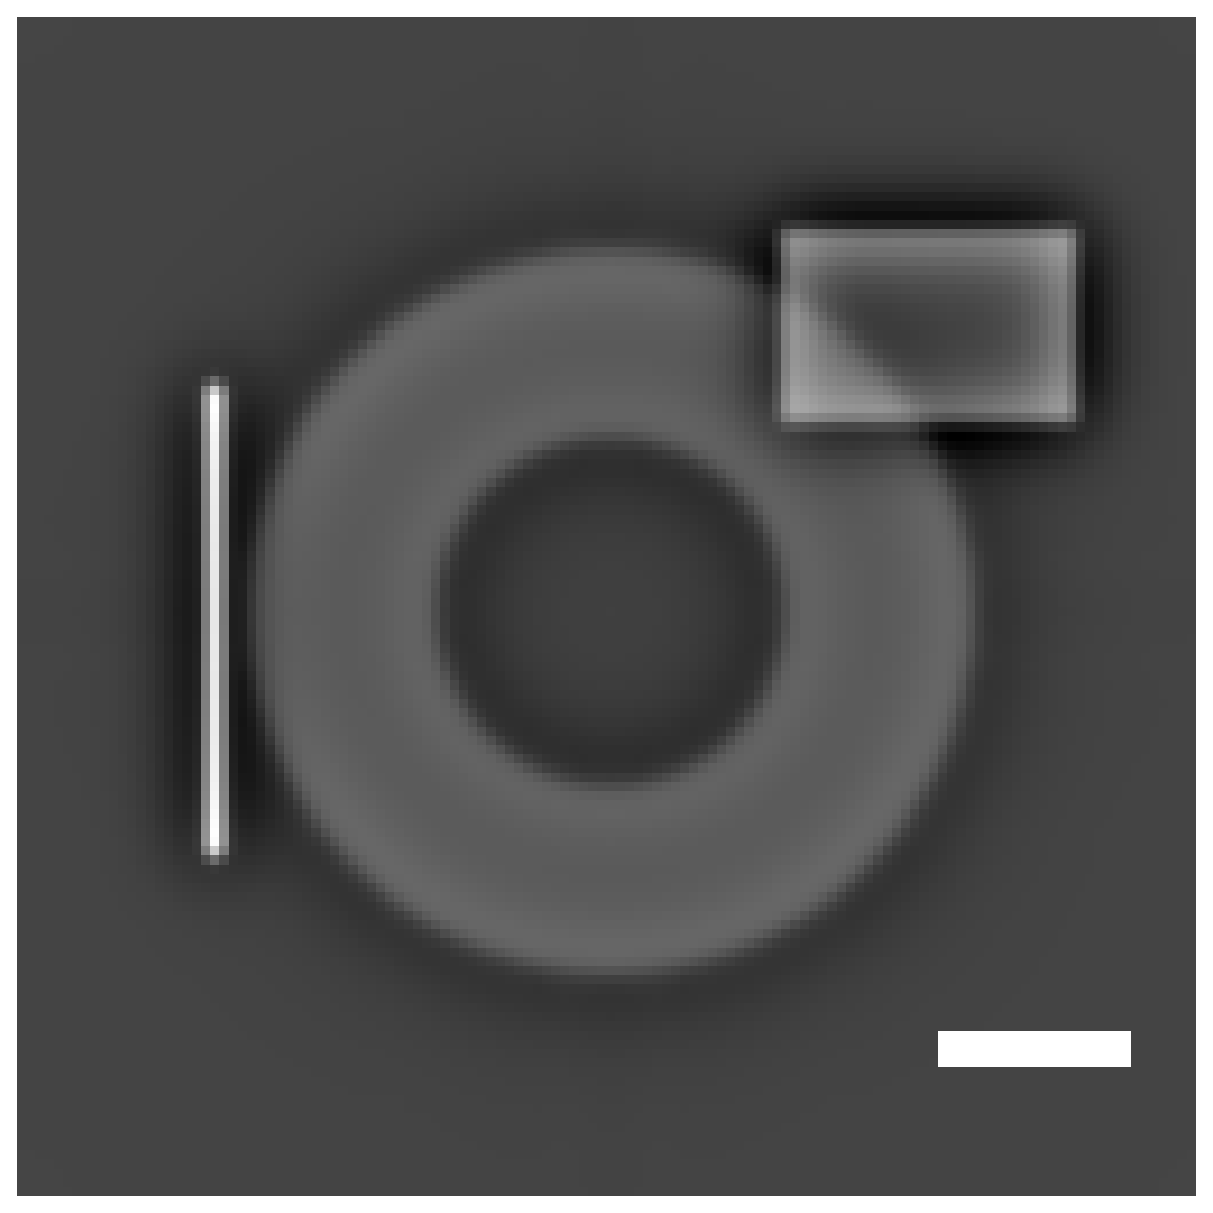
\includegraphics[width=4cm]{../app_hilo/ihp}}
  \subfigure[Combined images $\hat I_\textrm{hilo}$ in k-space.]{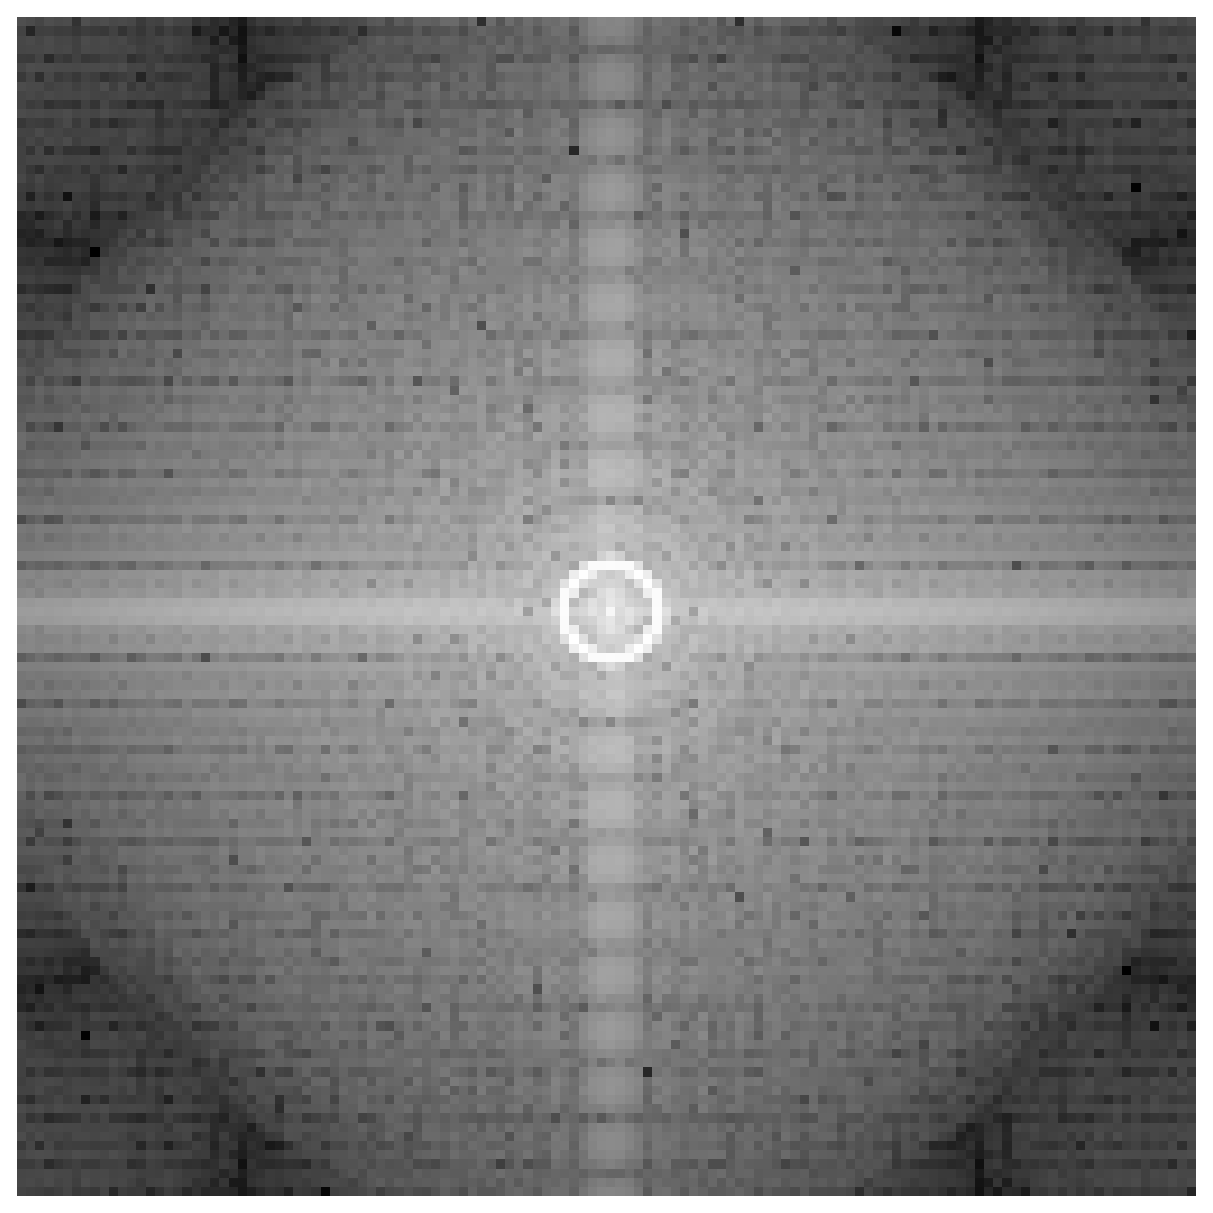
\includegraphics[width=4cm]{../app_hilo/kihilo}}
  \subfigure[Combined section $I_\textrm{hilo}$.]{\label{fig:ihilo}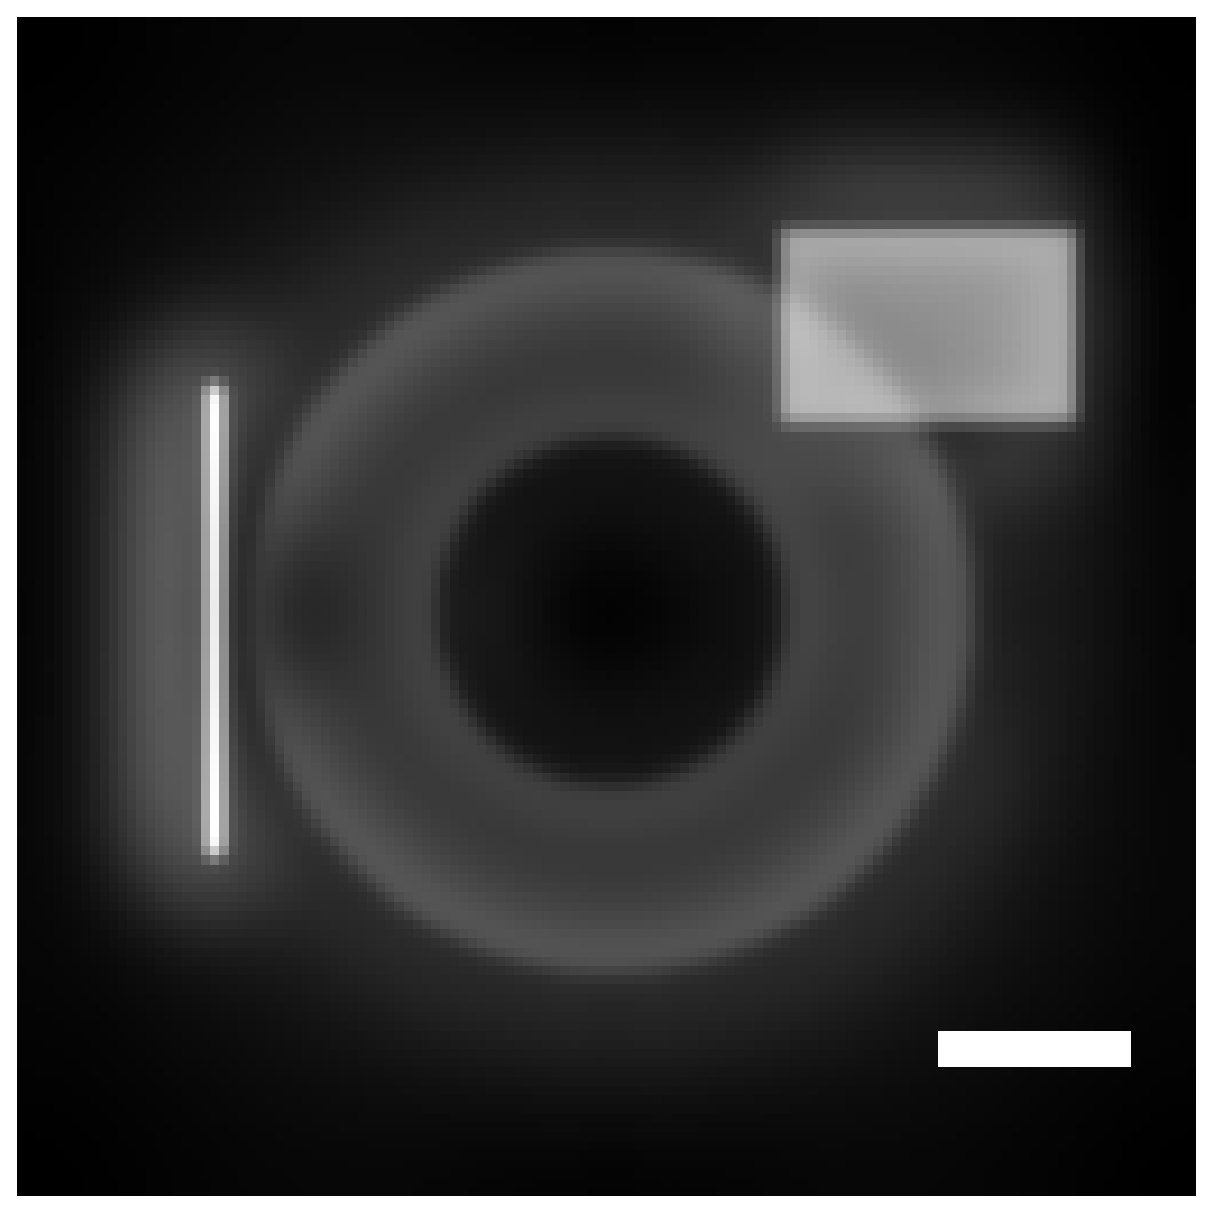
\includegraphics[width=4cm]{../app_hilo/ihilo}}
  \caption{Further intermediate and the end result of the HiLo ``speckle'' algorithm. The white circle in image {\bf (b)} marks $k_c$. The scalebars are \unit[2]{$\mu$m} wide.}
  \label{fig:hilo1interm2}
\end{figure}
%FIXME figure out unit of kc

\subsubsection*{Discussion}
This algorithm only requires that the illumination intensity in $I_n$
fluctuates over a certain region. Probably one gets better results
when the exact illumination pattern is known and taken into account.

\subsubsection{Grating}
The younger paper \cite{2009Santos} addresses this issue by using a
defined pattern in the excitation illumination. Instead of random
speckle a grating on a spatial light modulator is projected into the
specimen (giving actually images that resemble the simulated images in
this document).

Starting from a widefield image $I_u$ and an image $I_n$ that has been
illuminated with a grating they first determine the ratio $R=I_n/I_u$.
With equations \eqref{eqn:Iu} and \eqref{eqn:In} defining the
relationship between in-focus and out-of-focus light in both images it
follows:
\begin{align}
  R&=1+CM\sin(\kappa x+\varphi)),\\
  C&=\frac{I_\textrm{in}}{I_\textrm{in}-I_\textrm{out}}.
\end{align}
Here $C$ is the local image contrast (containing information similar
to $c_s$ in the HiLo ``speckle'' method) that is necessary to
determine the low-resolution sectioned image. The Fouriertransform
$\hat R$ (see \figref{fig:hatR}) of the ratio contains a peak in the
center (due to the constant 1) and at least two more peaks ($\pm 1$
order) on the $k_x$ axis. There are a strong $\pm 1$ order and a
weaker $\pm 2$ order as a rectangular grating is imaged into the
sample (as opposed to a Sine grating).
%FIXME the weak grating isn't in In! so maybe it is due to the ratio

To extract the modulated signal a filter is constructed that selects
only the first order on the right side of the Fouriertransform. The
result of the filter is shown in \figref{fig:hatR+}. The intermediate
image $I_{su}=\abs{R^+}I_u$ (see \figref{fig:isu2}) contains the
low-resolution sectioned image.

\begin{figure}[htb]
  \centering \subfigure[Ratio
  $R=I_n/I_u$.]{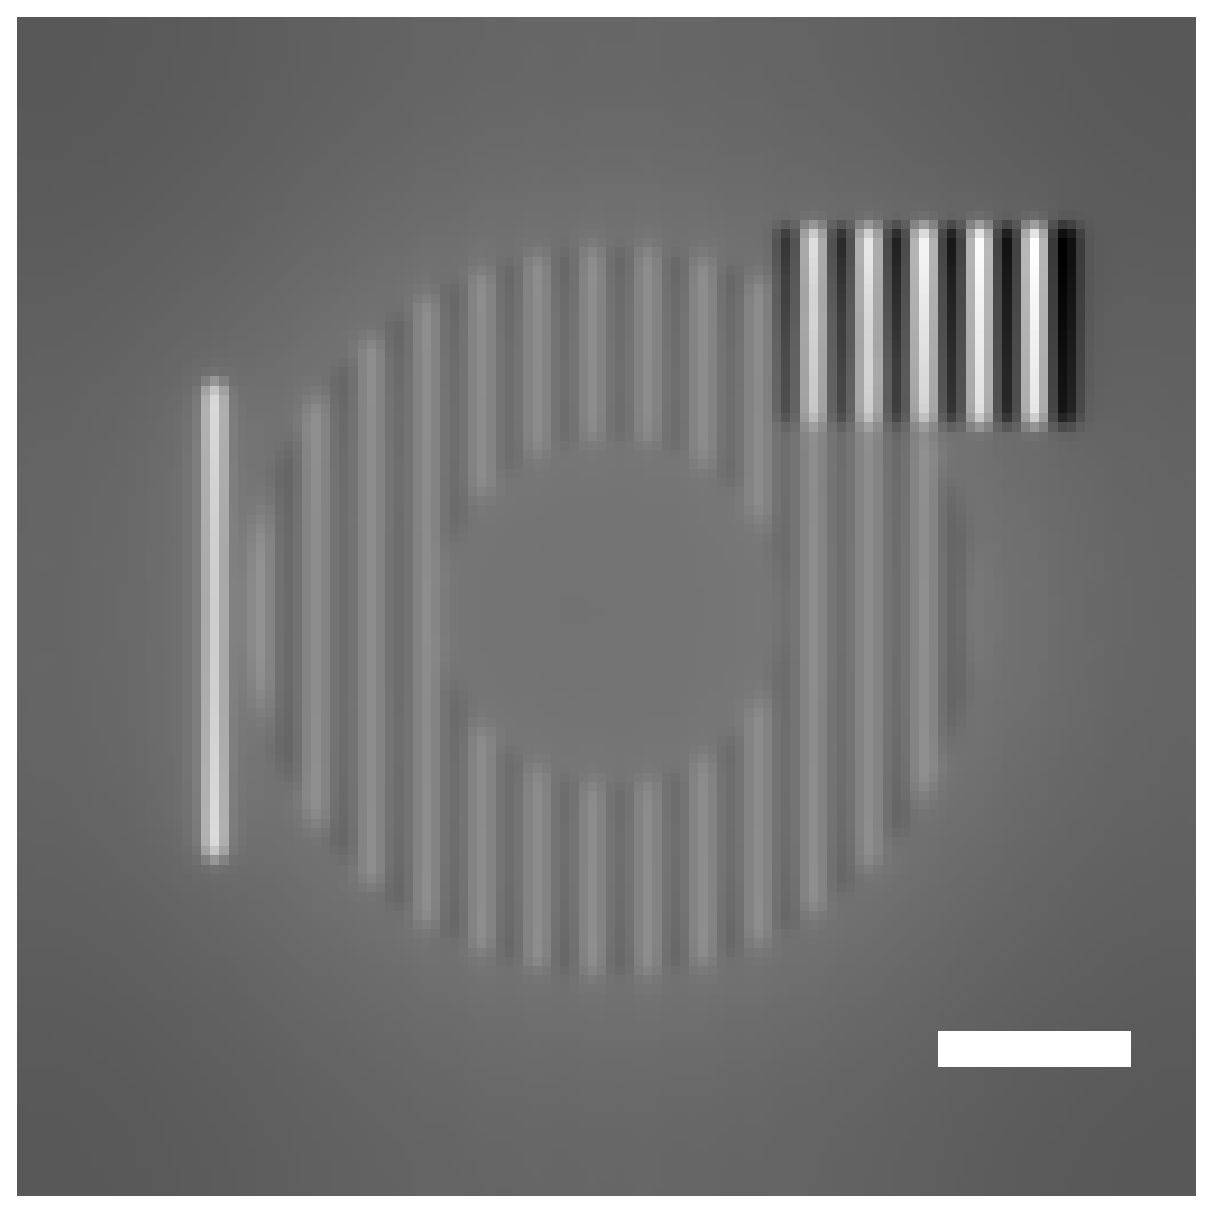
\includegraphics[width=4cm]{../app_hilo/ratio}}
  \subfigure[Fouriertransform $\hat
  R$.]{\label{fig:hatR}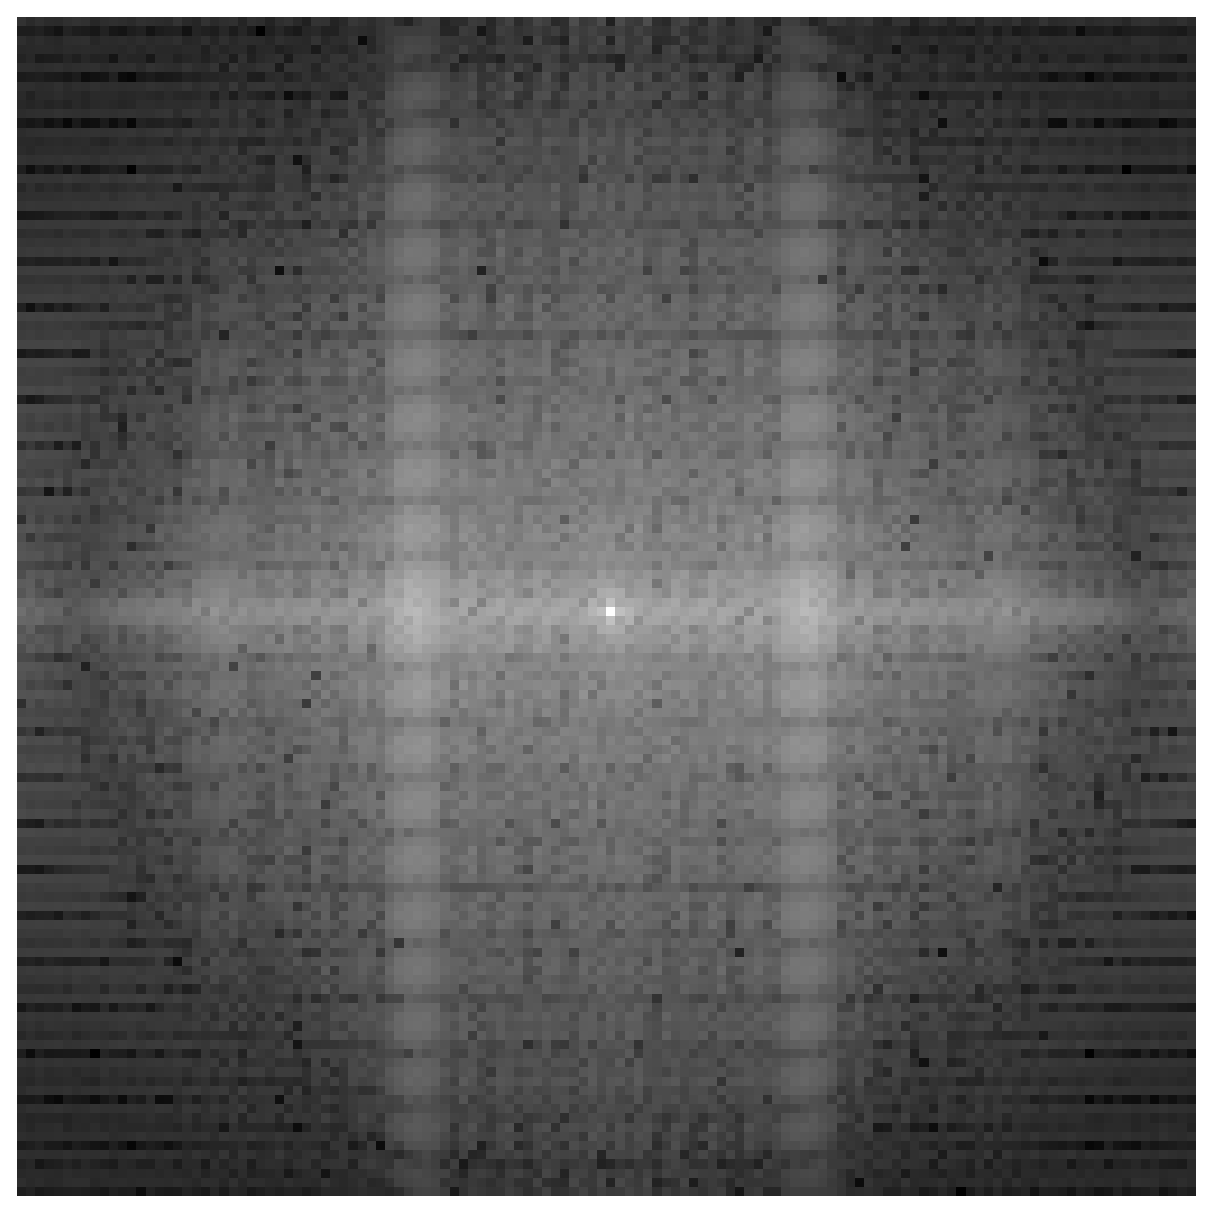
\includegraphics[width=4cm]{../app_hilo/ftratio}}
  \subfigure[Filtered first order $\hat
  R^+$.]{\label{fig:hatR+}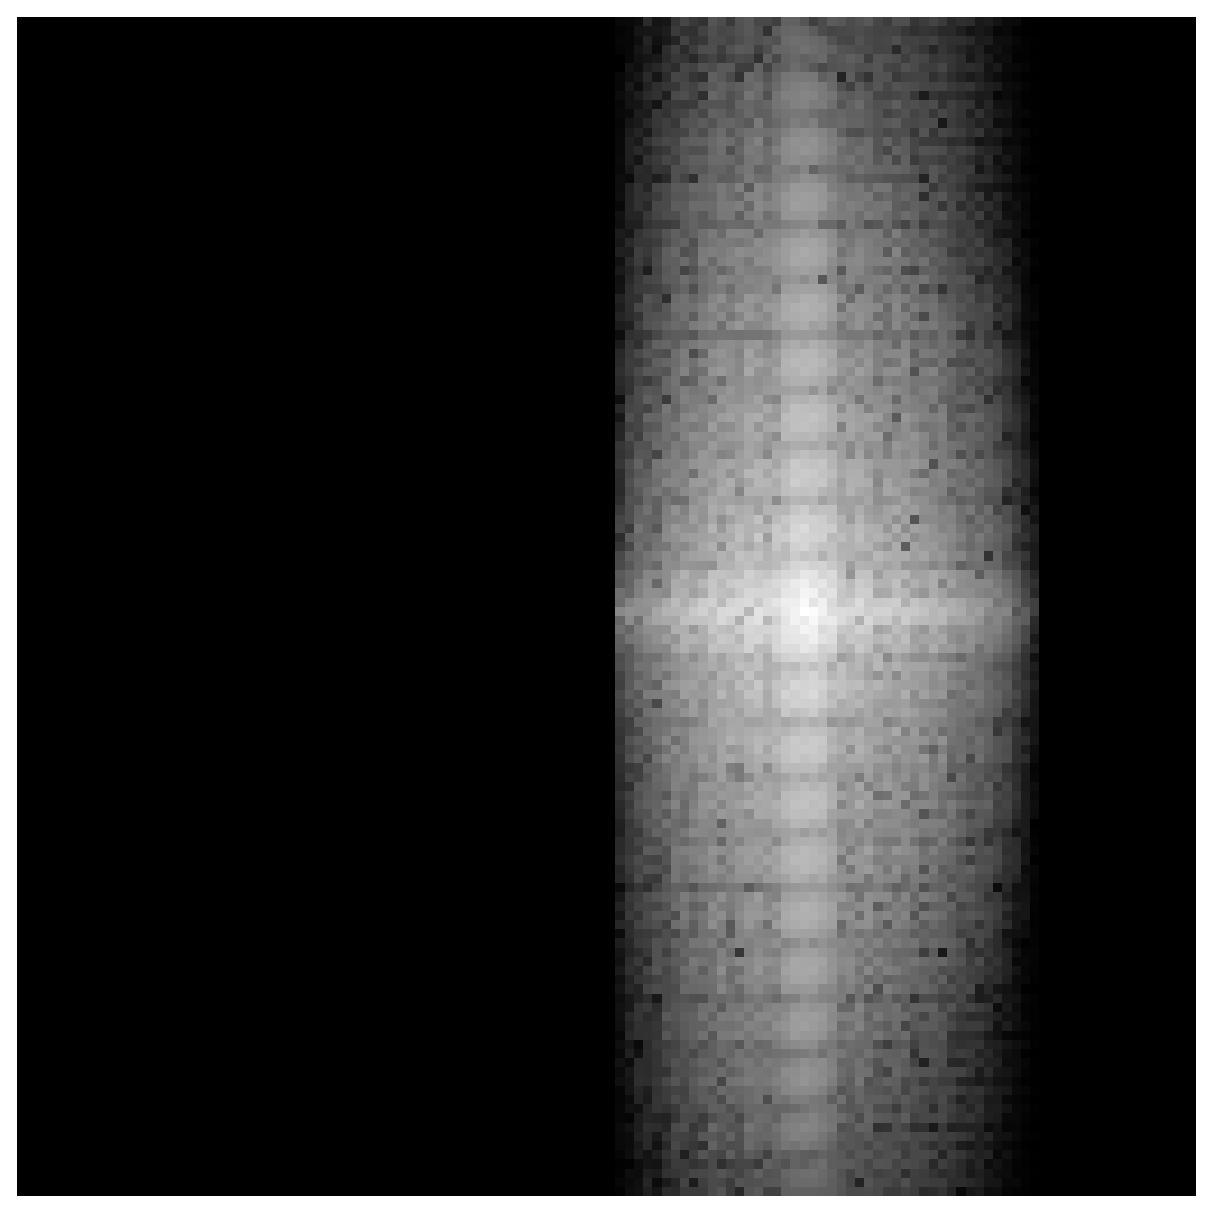
\includegraphics[width=4cm]{../app_hilo/filterftratio}}
  \caption{Intermediate results for the HiLo ``ratio'' algorithm. The scalebar in (a) is \unit[2]{$\mu$m} wide.}
  \label{fig:hilo2}
\end{figure}

The following listing shows the code for the algorithm:
\begin{lstlisting}
si=size(in);
n=si(1);
r=rr(in,'freq');
ratio=in./iu;
ft(ratio)
%% select R+ and construct isu
filter=gaussf((xx(in,'freq')>0.1) & (xx(in,'freq')<0.27),4);
ftratio=ft(ratio);
cm=abs(ift(filter.*ftratio));
isu=cm.*iu
%% calculate low pass filtered low-res section
kc=.07;
klp=exp(-r.^2/(2*kc^2));
ilp=real(ift(klp.*ft(isu)))
%% calculate high pass filtered high-res section
ihp=real(ift((1-klp).*ft(iu)))
%% construct the circle for integration in k-space
ring=abs(ft(besselj(0,2*pi*kc*n.*r)));
ring2=r-1./n<kc & r+1./n>kc;
cring=ring.*ring2;
nring=cring./sum(abs(cring))
%% do the integration
eta=sum(abs(ft(ihp))/abs(ft(ilp)).*nring)
%% combine section
ihilo=eta.*ilp+ihp
\end{lstlisting}

I chose the cutoff frequency $k_c$ high enough so that $I_\textrm{lp}$
doesn't look too smooth but also low enough so that I don't loose too
much information from the $I_\textrm{hp}$ image. The scale factor
$\eta$ for $I_\textrm{lp}$ and $I_\textrm{hp}$ is calculated as in the
previous section. Finally the combined sectioned image is displayed in
\figref{fig:ihilo2}.

\begin{figure}[htb]
  \centering
  \subfigure[$I_{su}$]{\label{fig:isu2}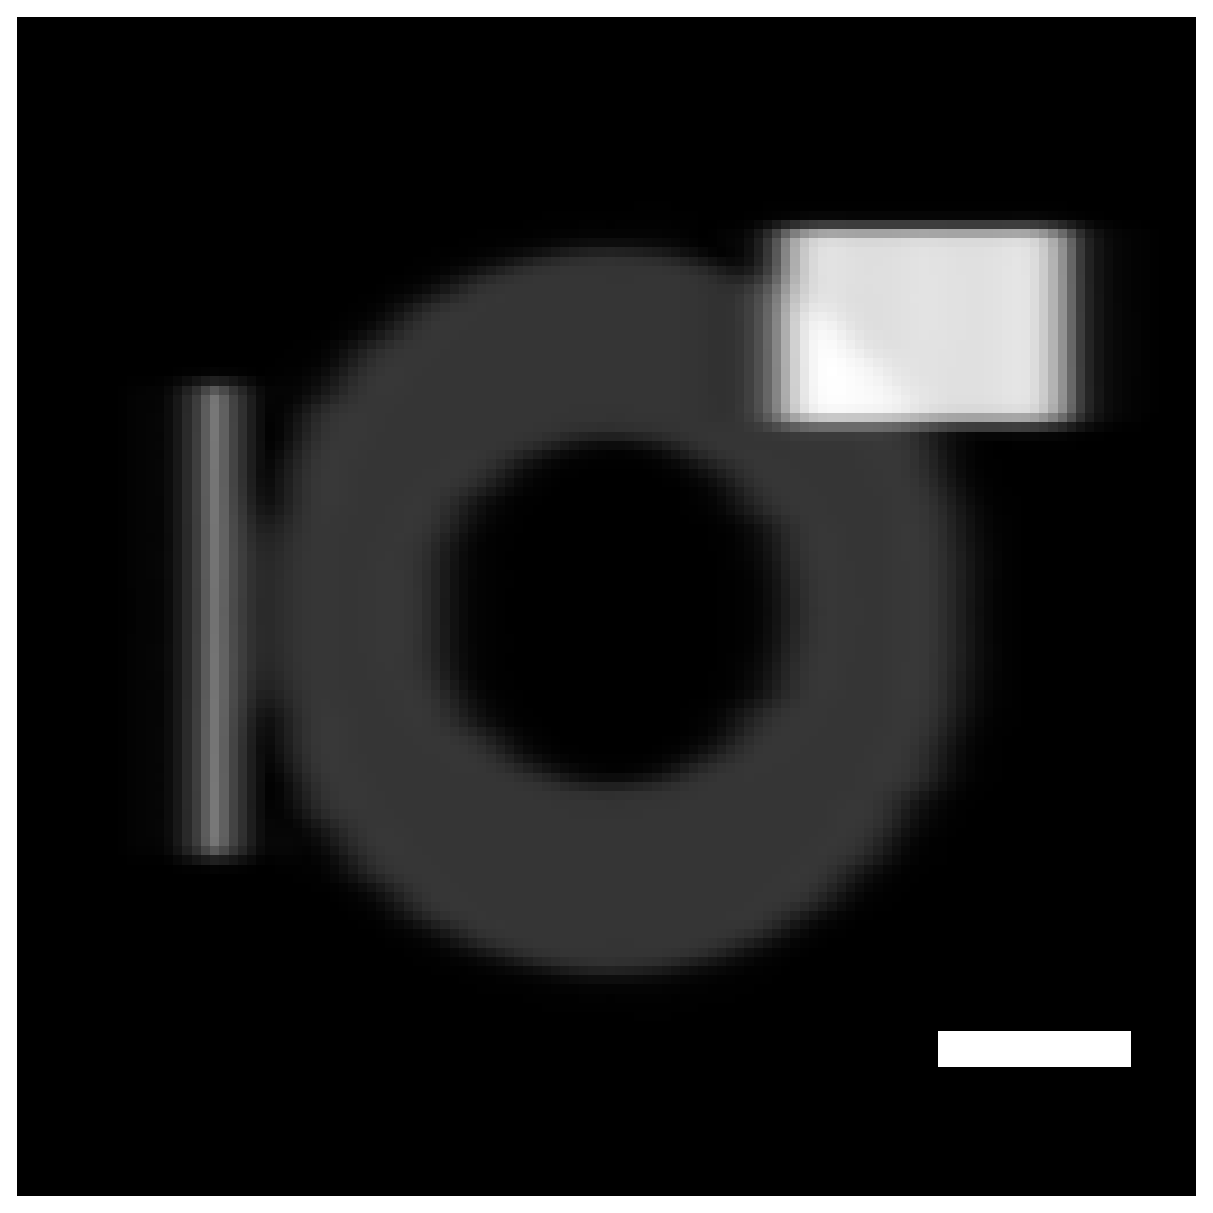
\includegraphics[width=4cm]{../app_hilo/isu2}}
  \subfigure[$I_\textrm{lp}$]{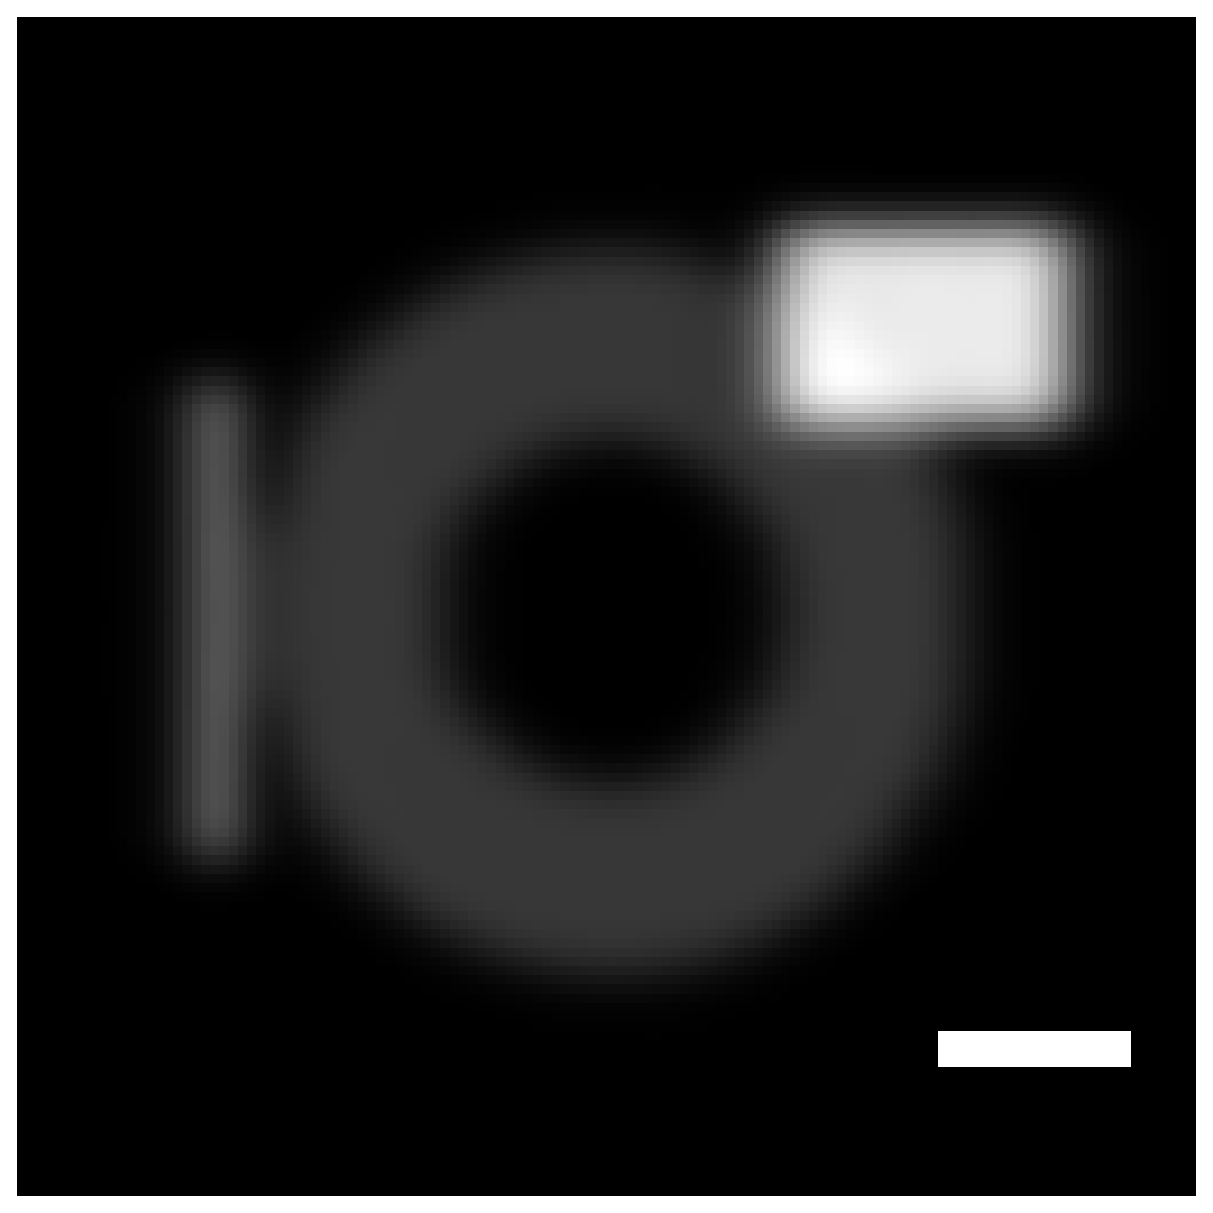
\includegraphics[width=4cm]{../app_hilo/ilp2}}
  \subfigure[$I_\textrm{hilo}$]{\label{fig:ihilo2}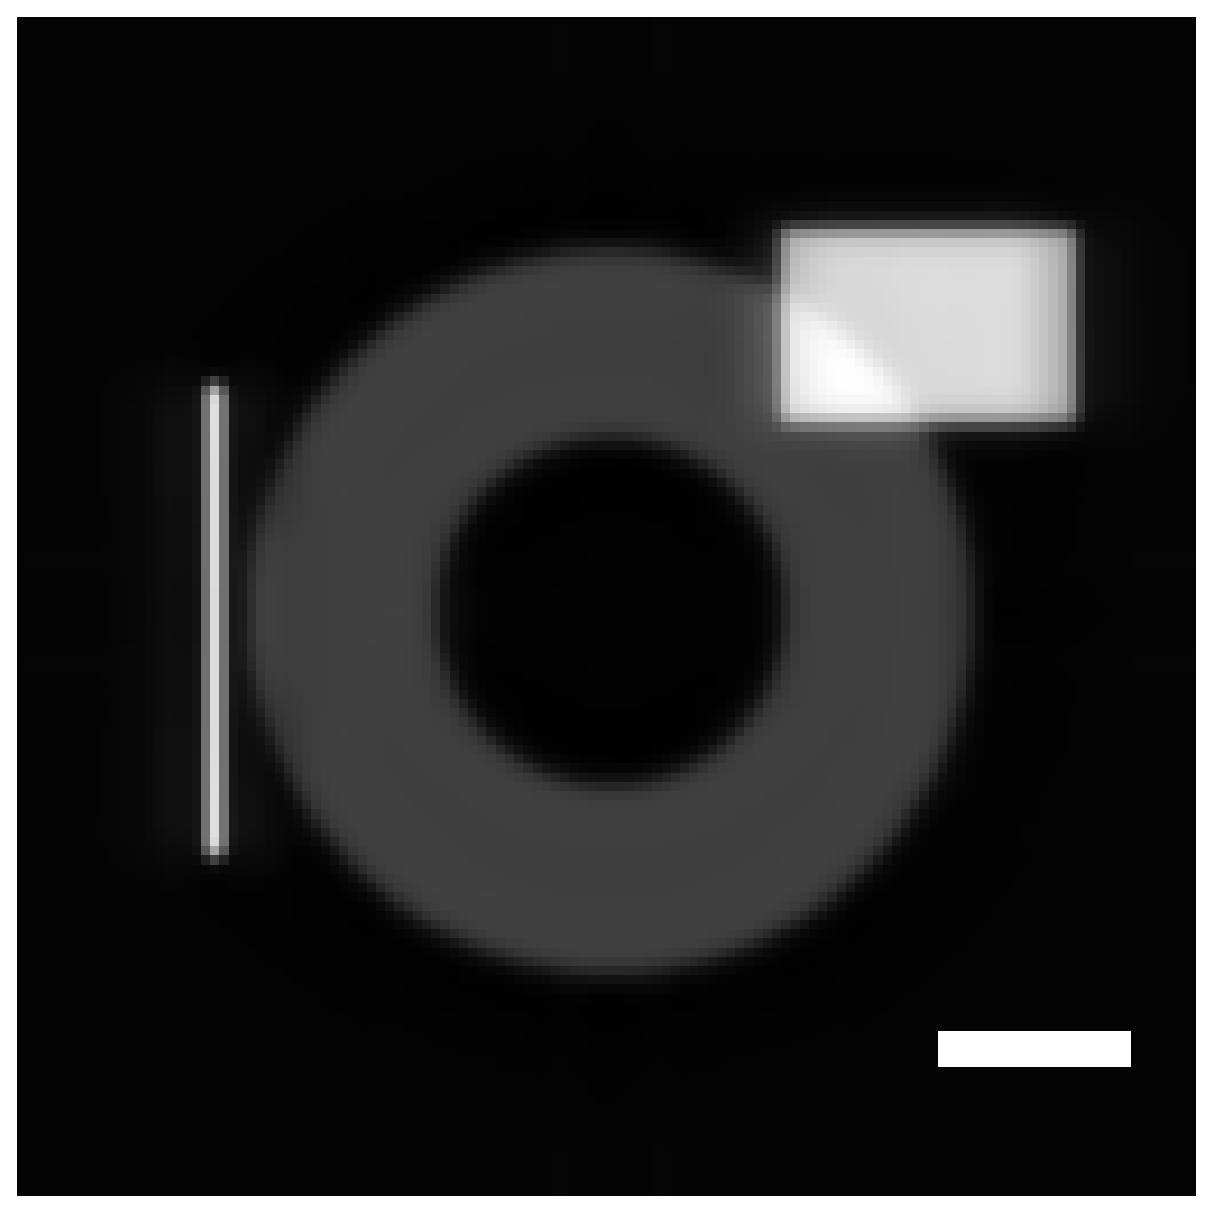
\includegraphics[width=4cm]{../app_hilo/ihilo2}}
  \caption{Intermediate results and the end result for the HiLo
    ``ratio'' algorithm. The scalebars are \unit[2]{$\mu$m} wide.}
  \label{fig:hilo2_2}
\end{figure}
\subsubsection*{Discussion}
One advantage of the ``ratio'' method compared to the ``speckle''
method is that it allows for a higher cut-off frequency $k_c$ without
introducing artifacts in the intermediate image $I_{su}$. That
accounts for the better appearance of the result \figref{fig:ihilo2}
compared to \figref{fig:ihilo} (at least for this particular grating).


Another thing that comes to mind is that the calculation of the ratio
isn't the only way to extract the modulated signal. Another approach
would involve subtracting the widefield image and shifting in fourier
space (discussion with Rainer Heintzmann). This will be discussed in
the following section.
\section{New Method}
Instead of using a non-hermitian filter to extract the modulated part
of the non-uniformly illuminated image $I_n$ it is also possible to
employ the Fourier shift theorem: A shift in real space is a
multiplication with a phase factor in k-space. 

Lets say we have two images $f(\vect x)$ and $g(\vect x)$. The image
$g$ contains the same information as $f$ but shifted by a vector
$\vect a$. The theorem can be expressed like this:
\begin{align}
  g(\vect x)=f(\vect x+\vect a)
  \quad
  \rightarrow
  \quad
  \hat g(\vect k)=e^{i\vect k\vect a}\hat f(\vect k).
\end{align}
One can find the shift by searching for the maximum $\vect x_0=\vect a$ in
the cross-correlation $cov(\vect x)$:
\begin{align}
  cov(f,g)(\vect x)
  =\int f(\vect\chi) g(\vect x+\vect\chi) \textrm{d}\vect\chi
  =f(\vect x)\otimes g(-\vect x)
  =FT^{-1}(\hat f(\vect k)\cdot\hat g^*(\vect k)).
\end{align}
First $I_u$ is subtracted from $I_n$ in order to suppress the zero
order. The following code integrates over a circle on the zero order
to find a constant {\tt kappa} to scale $I_u$ with. Furthermore the
Fouriertransform of the images is divided by the OTF in order to
correct for the non-constant frequency transfer in the micro objective.

\begin{lstlisting}
kin=ft(in);
kiu=ft(iu);
% scale kin and kiu so that ic has no zero order
kappa=sum(abs(kin)./abs(kiu).*(rr(in)<5))./sum(rr(in)<5)
%% project otf along z
skpsf=squeeze(sum(kpsf,[],3));
corr=gaussf((rr(skpsf,'freq')<.42),3)./skpsf;
%% correct for the otf
ckin=corr.*kin;
ckiu=corr.*kiu;
%% correlate to find grating positions
ackin=abs(ckin-kappa.*ckiu);
ackiu=abs(ckiu).*(rr(ackiu,'freq')<.16 | abs(xx(ackiu,'freq'))<.06);
\end{lstlisting}
The Fouriertransform of the OTF-corrected non-uniform image is shown
in \figref{fig:ackin}. It still contains the $\pm1$ orders. In order
to measure their exact position (depending on grating period {\tt P})
the ``interesting'' bit of the widefield k-space is selected (in
variable {\tt ackiu}) and cross-correlated with {\tt ackin}.

\begin{figure}[htb]
  \centering \subfigure[{\tt
    ackin}]{\label{fig:ackin}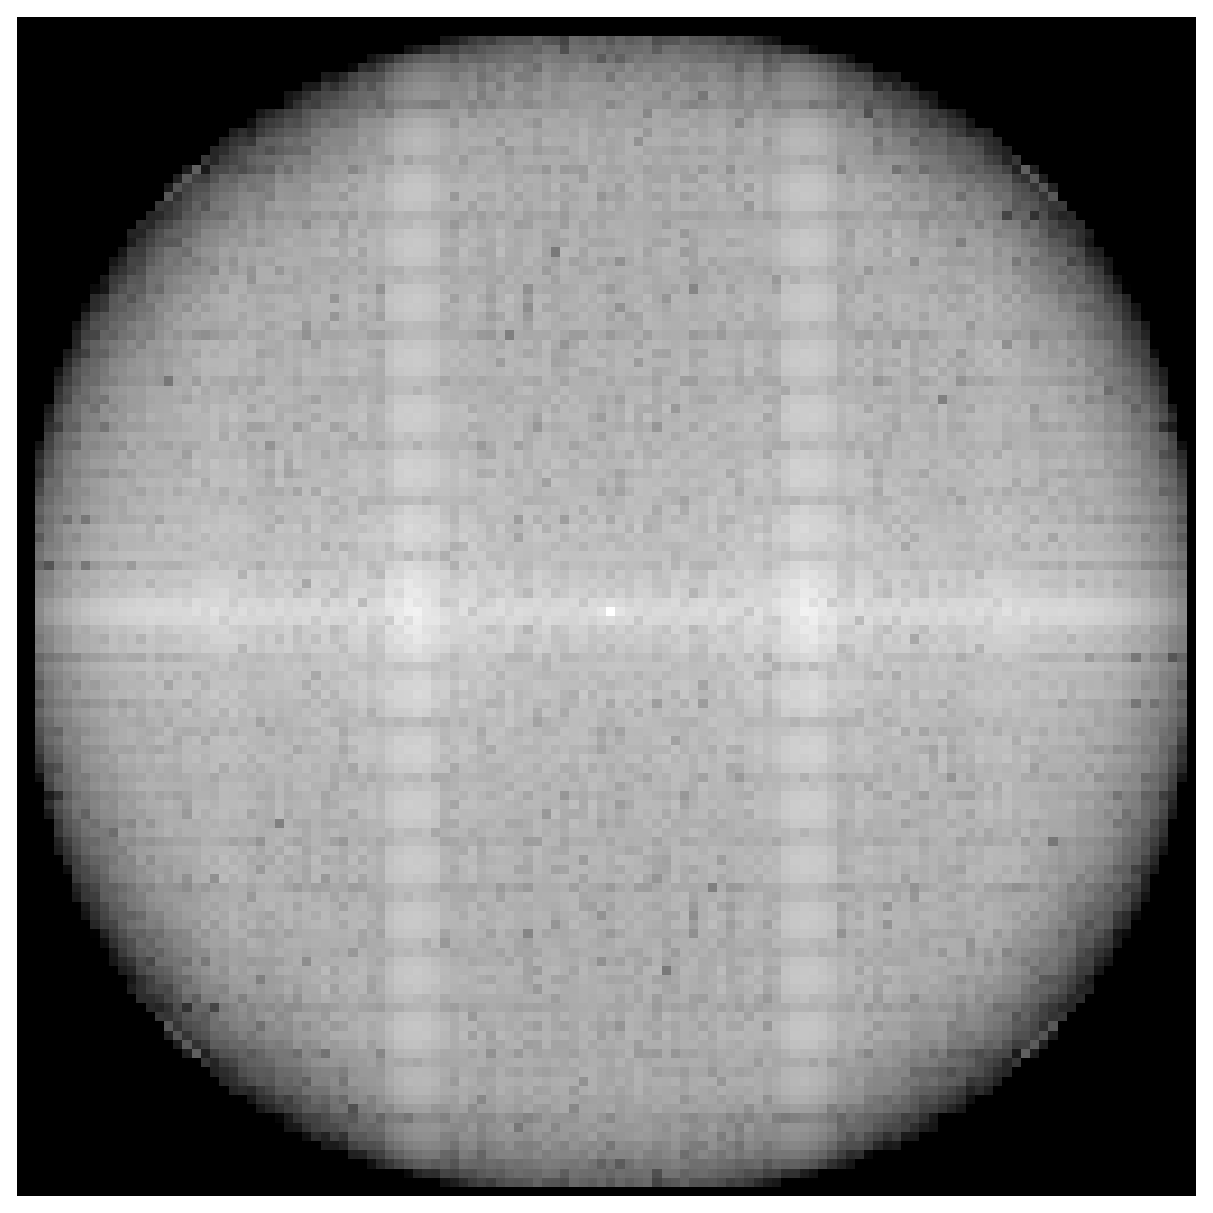
\includegraphics[width=6cm]{../app_hilo/ackin}}
  \subfigure[{\tt
    ackiu}]{\label{fig:ackiu}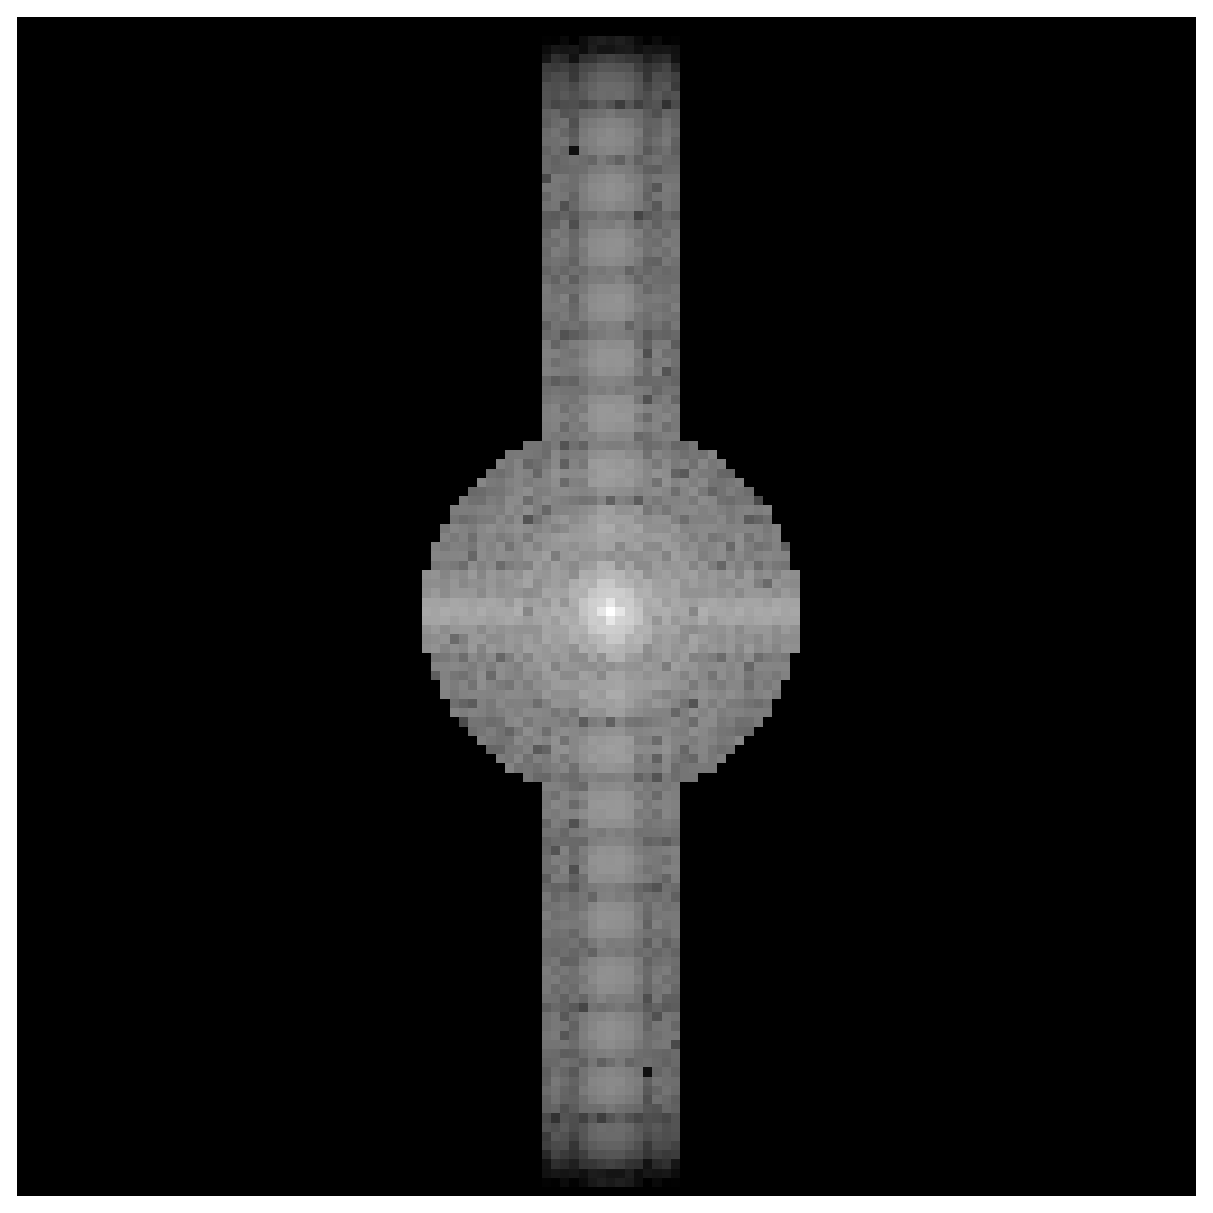
\includegraphics[width=6cm]{../app_hilo/ackiu}}
  \subfigure[Cross correlation
  $cov$.]{\label{fig:cov}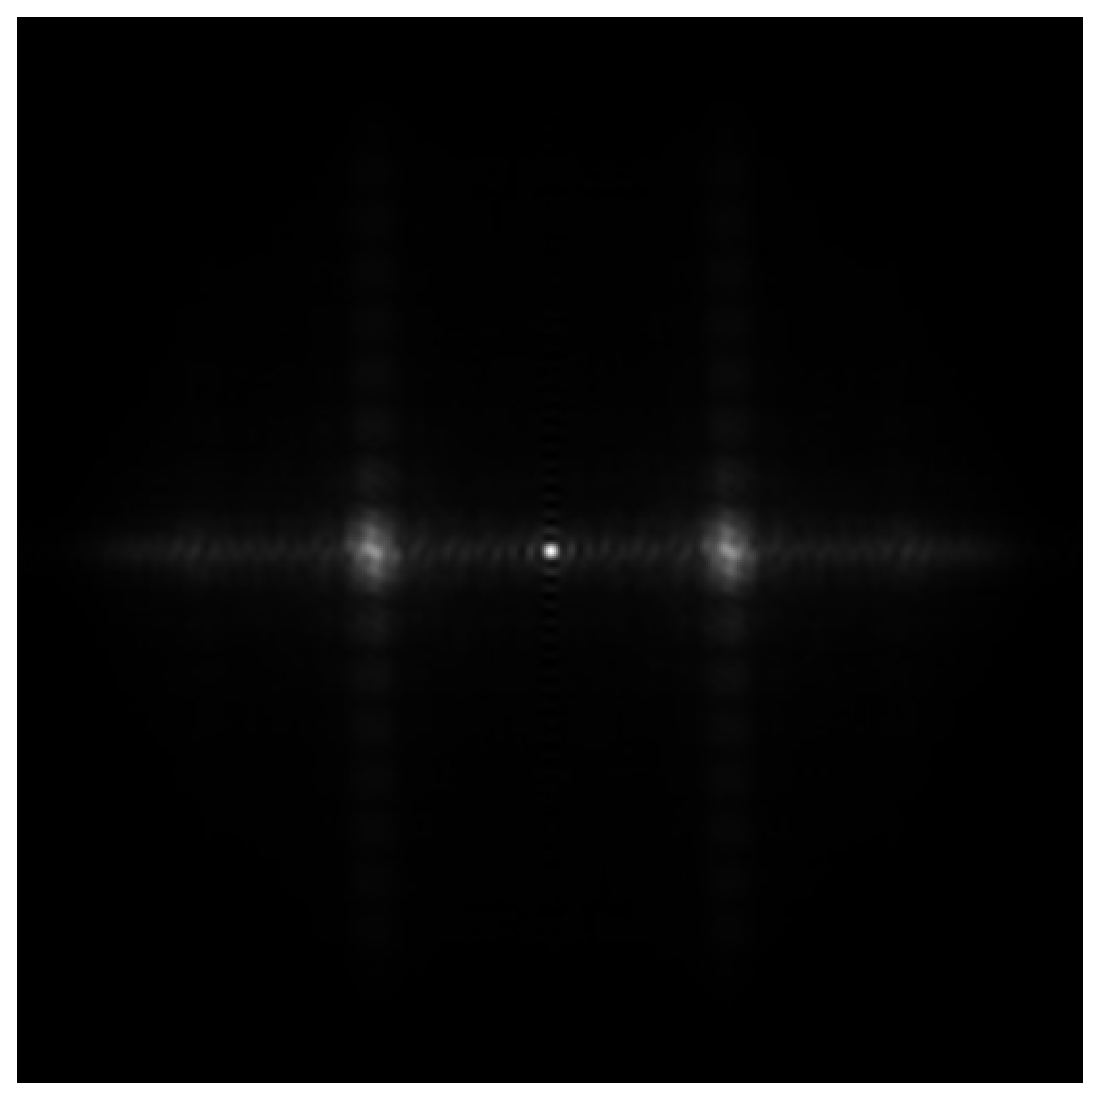
\includegraphics[width=6cm]{../app_hilo/cov}}
  \subfigure[Surface plot of
  $cov$.]{\label{fig:cov3d}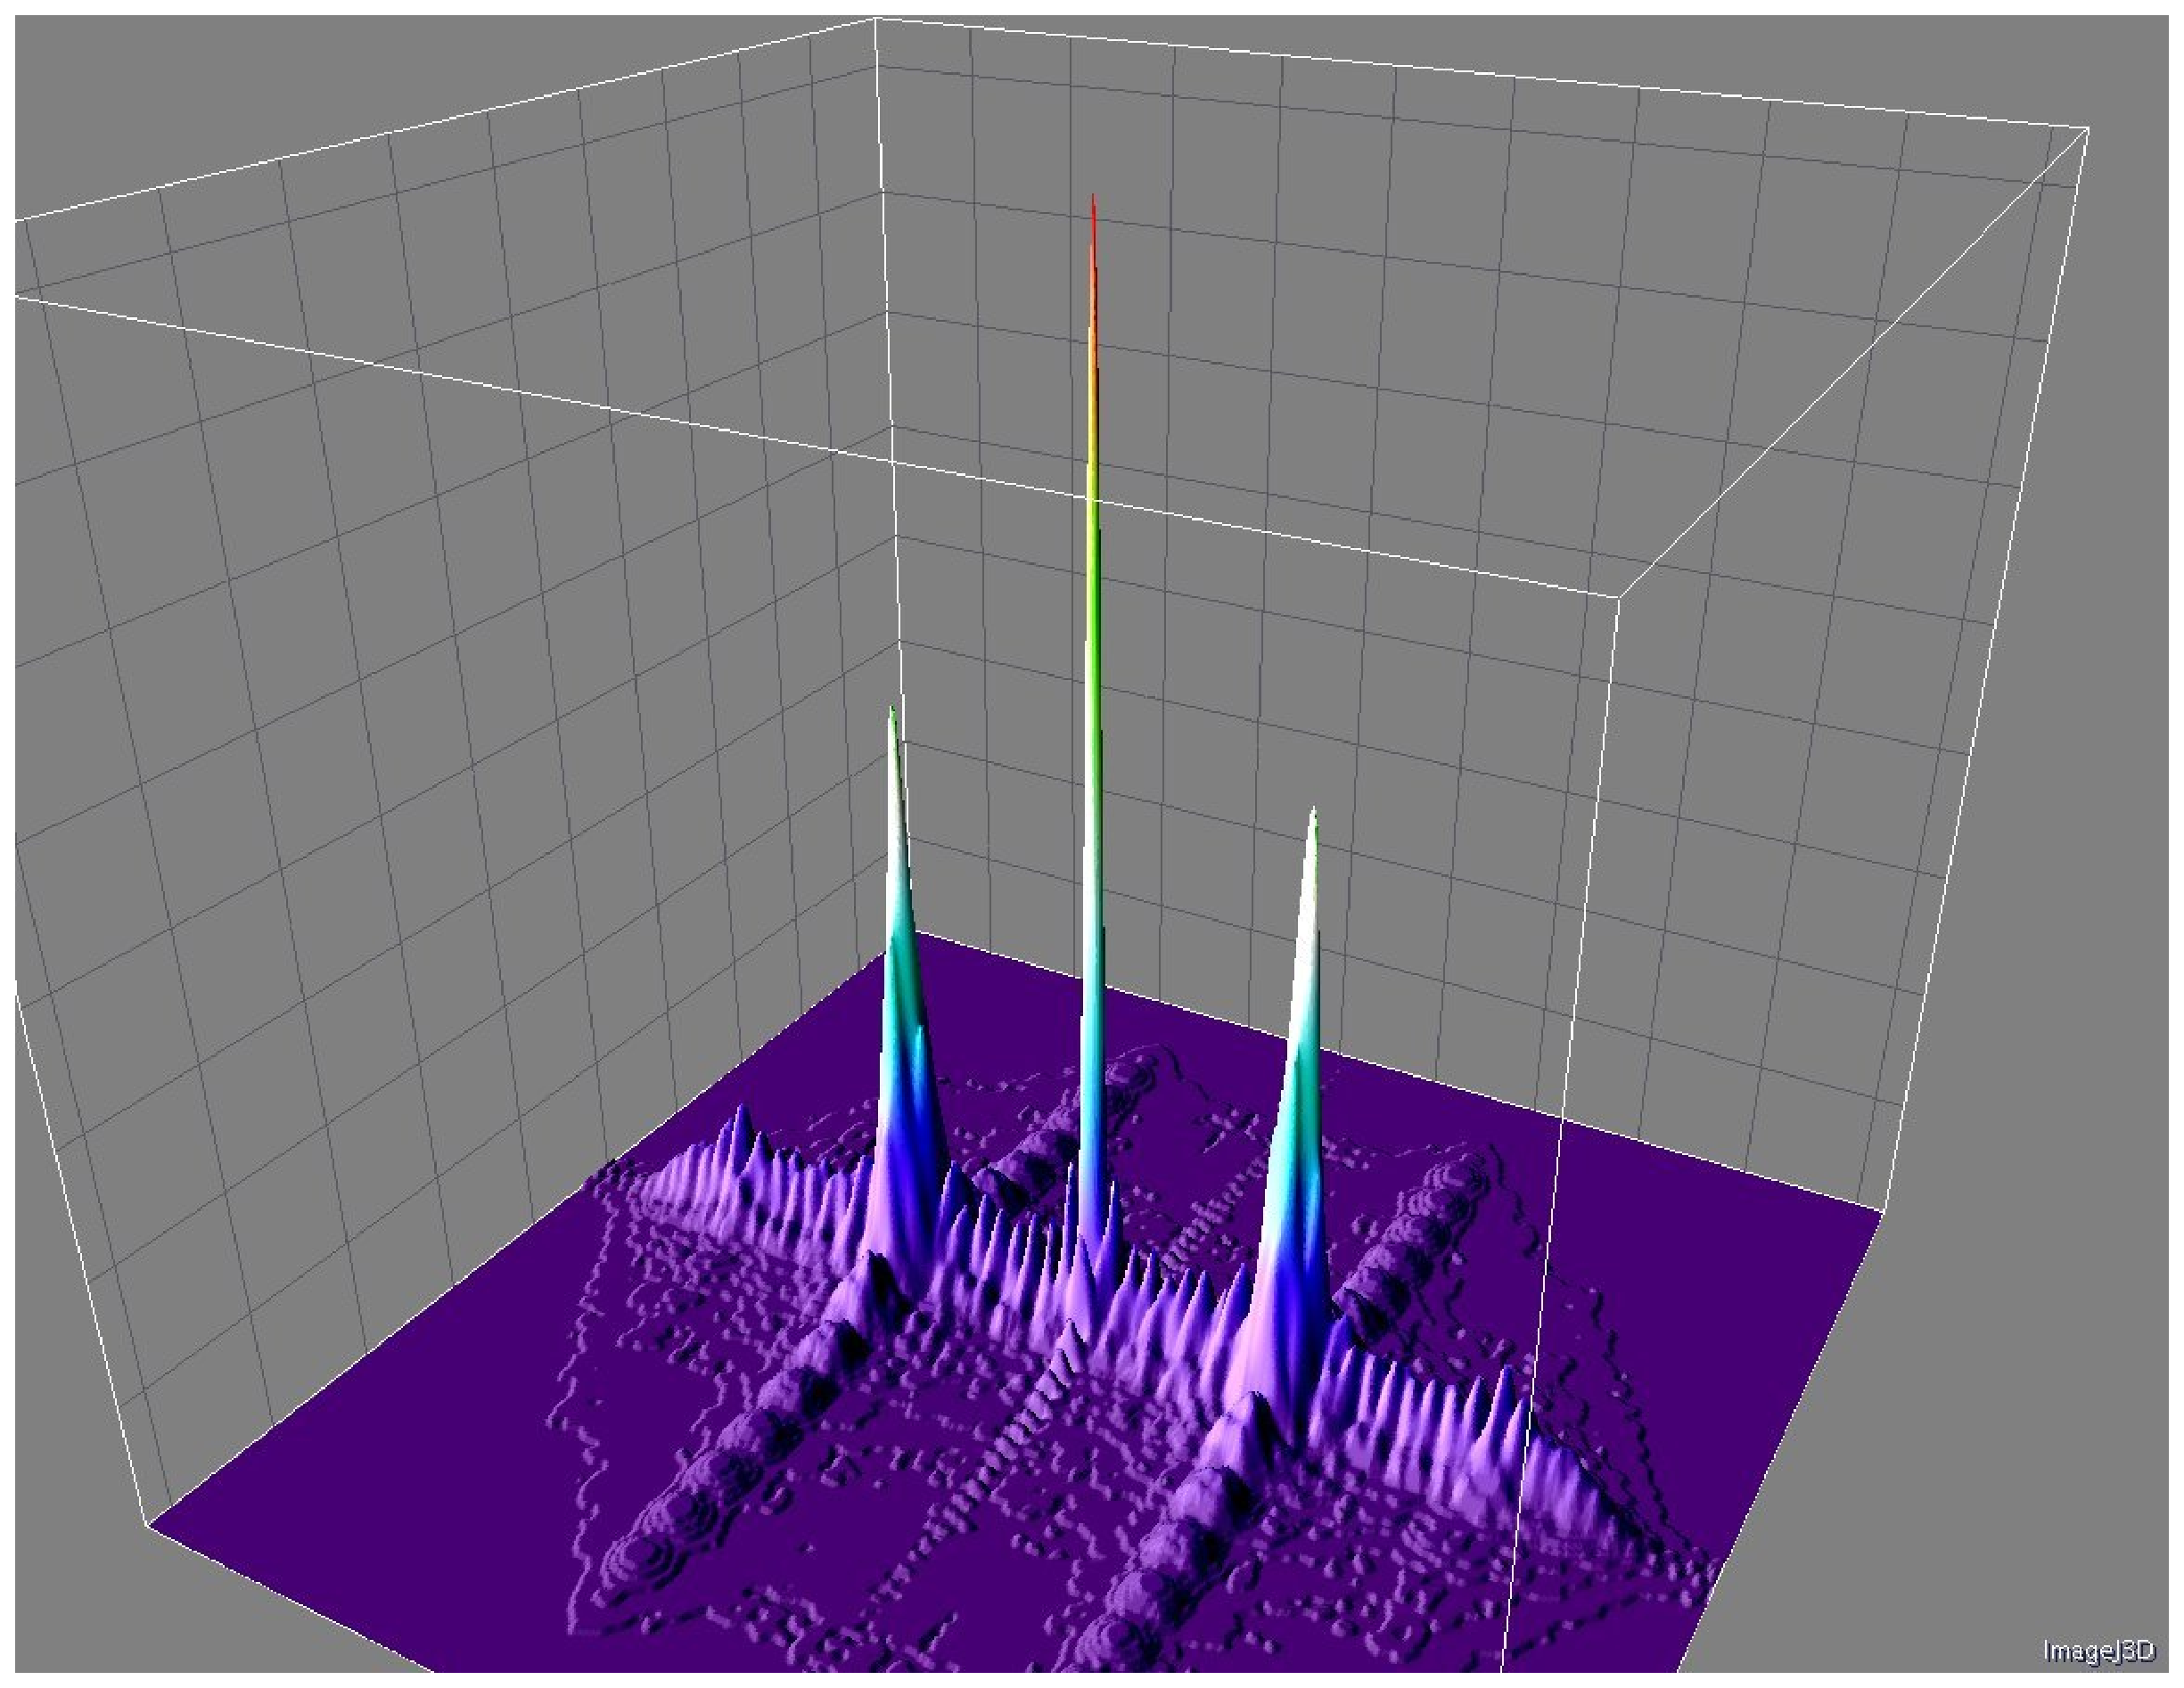
\includegraphics[width=6cm,viewport=100 0 920
    820,clip]{../app_hilo/cov3d}}
  \caption{Intermediate results for our HiLo ``shift'' algorithm.}
  \label{fig:hilo3}
\end{figure}

In order to locate the maximum in the cross-correlation with a high
enough accuracy the convolution is done on a finer grid by
zero-padding the input images as shown in the following listing: 
\begin{lstlisting}
kcov=ft(ackin).*conj(ft(ackiu));
kcov_big=newim(512,512)+i-i; % subsample the correlation by zero padding
st=256-64; w=127; en=st+w;
kcov_big(st:en,st:en)=kcov;
cov=abs(ift(kcov_big)); % this contains the cross correlation
\end{lstlisting}
The $512\times512$ image {\tt cov} is shown in \figref{fig:cov} and
\figref{fig:cov3d}. The next listing is the code to locate the center of gravity of the nine points on top of the right peak:
\begin{lstlisting}
%% find maximum on the right of the correlation
startx=75*4;
[m,p]=max(abs(cov(startx:end,:)));
pos=[p(1)+startx,p(2)];
% determine center of mass of the 3x3 region around the maximum
region=abs(cov(pos(1)-1:pos(1)+1,pos(2)-1:pos(2)+1));
region=region-min(region);
cm=[sum(xx(region).*region),sum(yy(region).*region)];
shift=(pos+cm-[256,256])/4 % divide by 4 to undo subsampling
\end{lstlisting}
For the example the displacement {\tt shift} is $(21.25,0)$ relative
to the center of the $128\times128$ image.

\begin{figure}[htb]
  \centering \subfigure[ $\hat
  q_s$.]{\label{fig:kqs}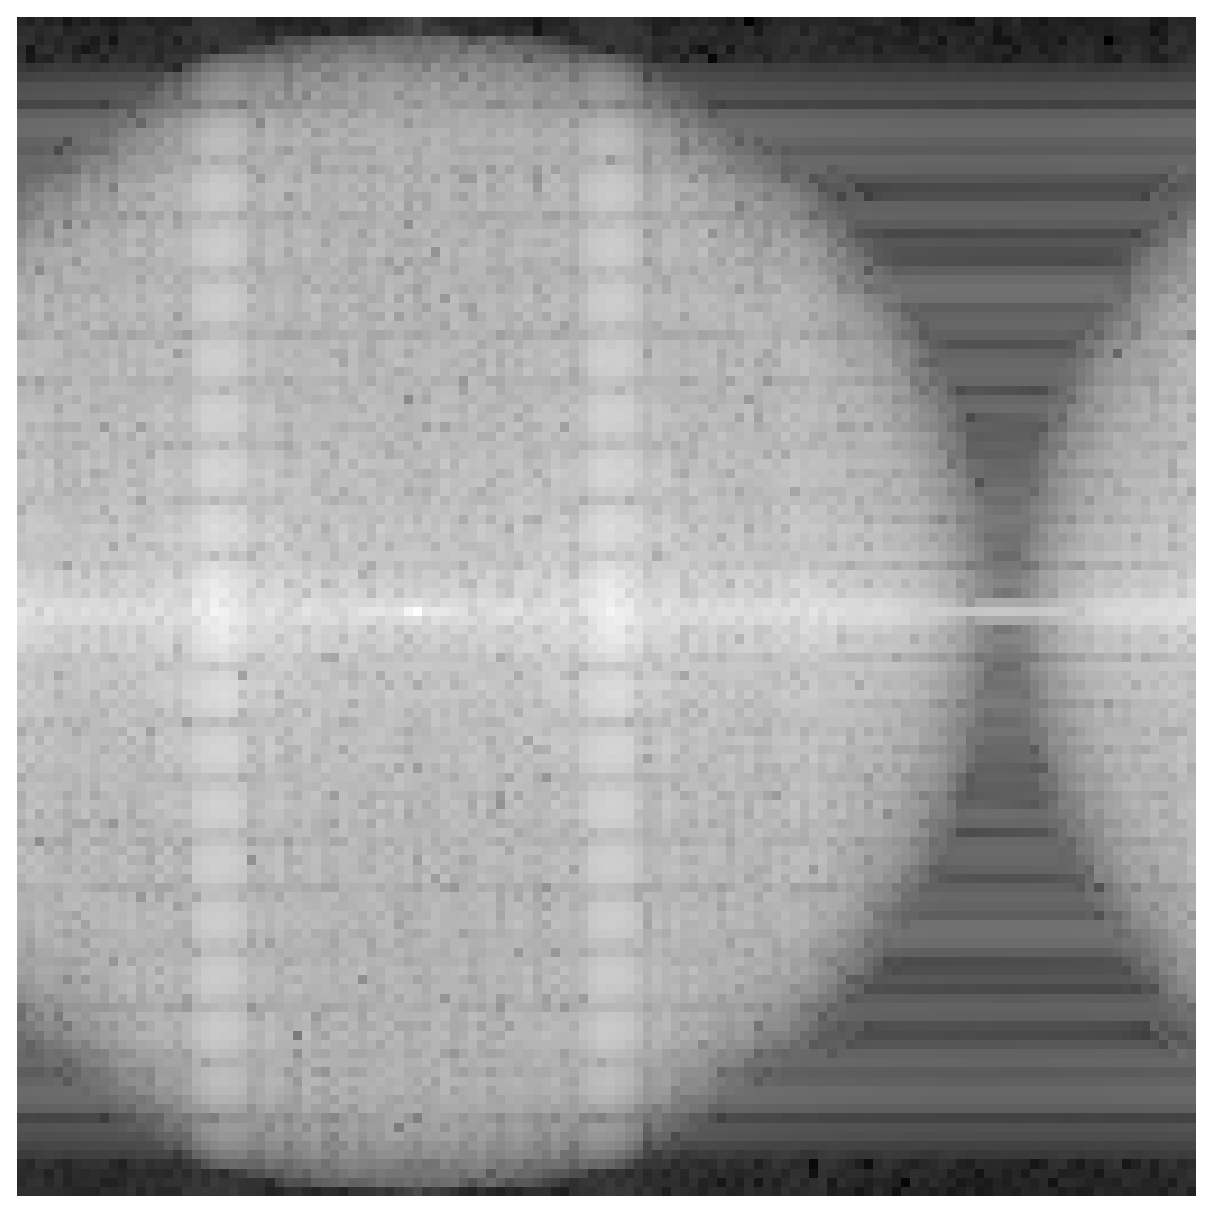
\includegraphics[width=4cm]{../app_hilo/kqs}}
  \subfigure[$\hat q_s$ with low-pass
  applied.]{\label{fig:kqslp}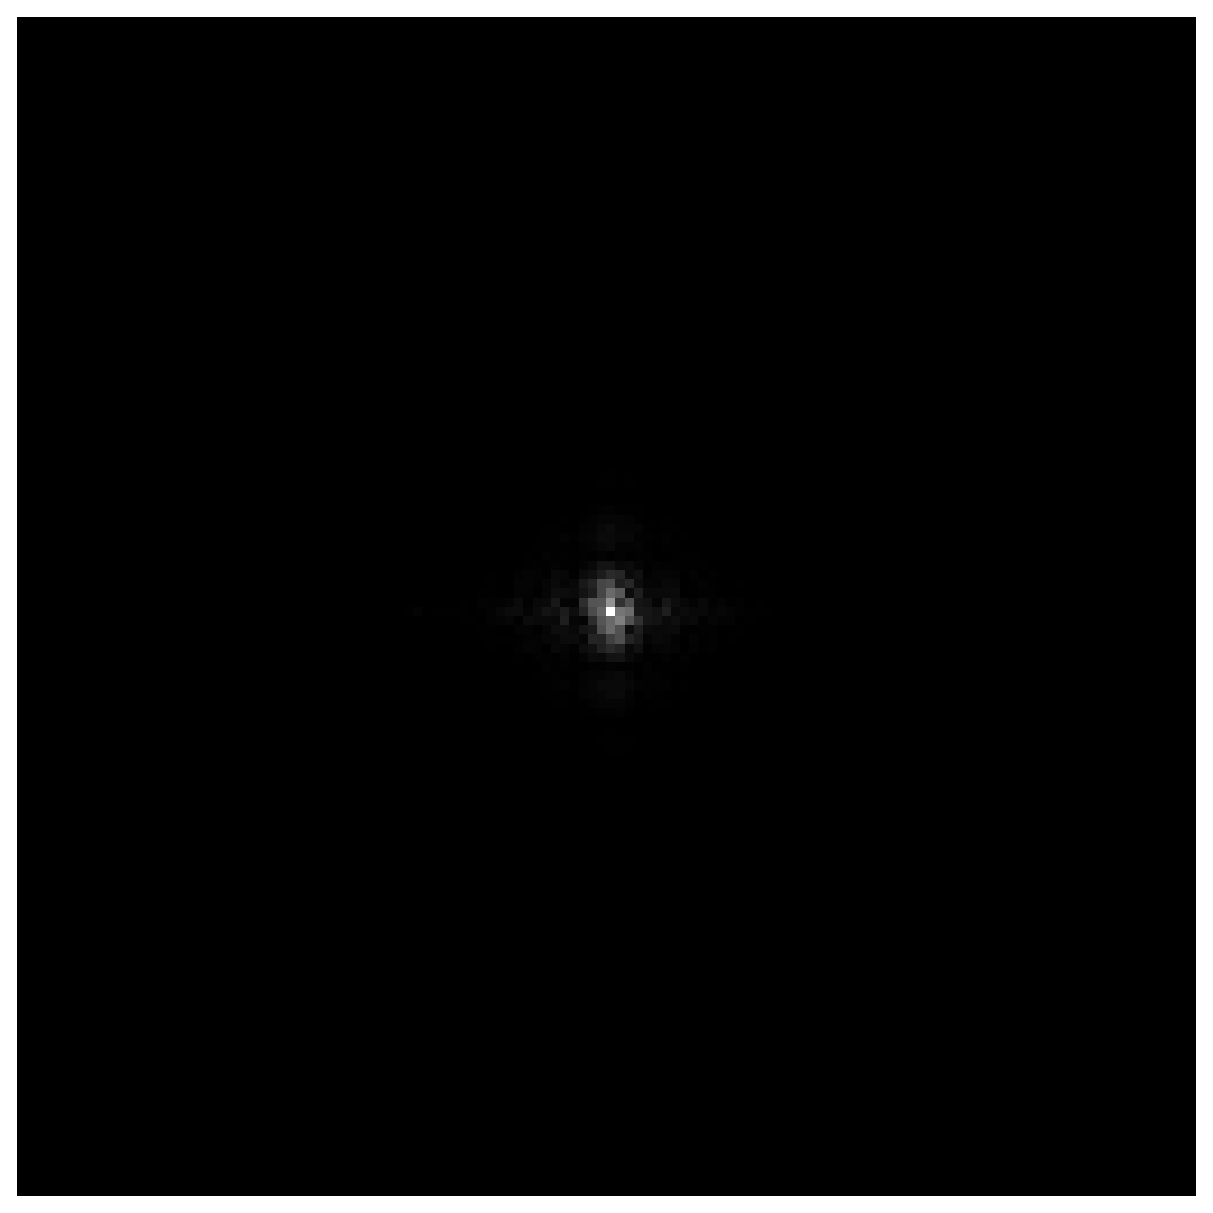
\includegraphics[width=4cm]{../app_hilo/kqslp}}
  \subfigure[$\hat
  I_\textrm{hp}$]{\label{fig:kihp3}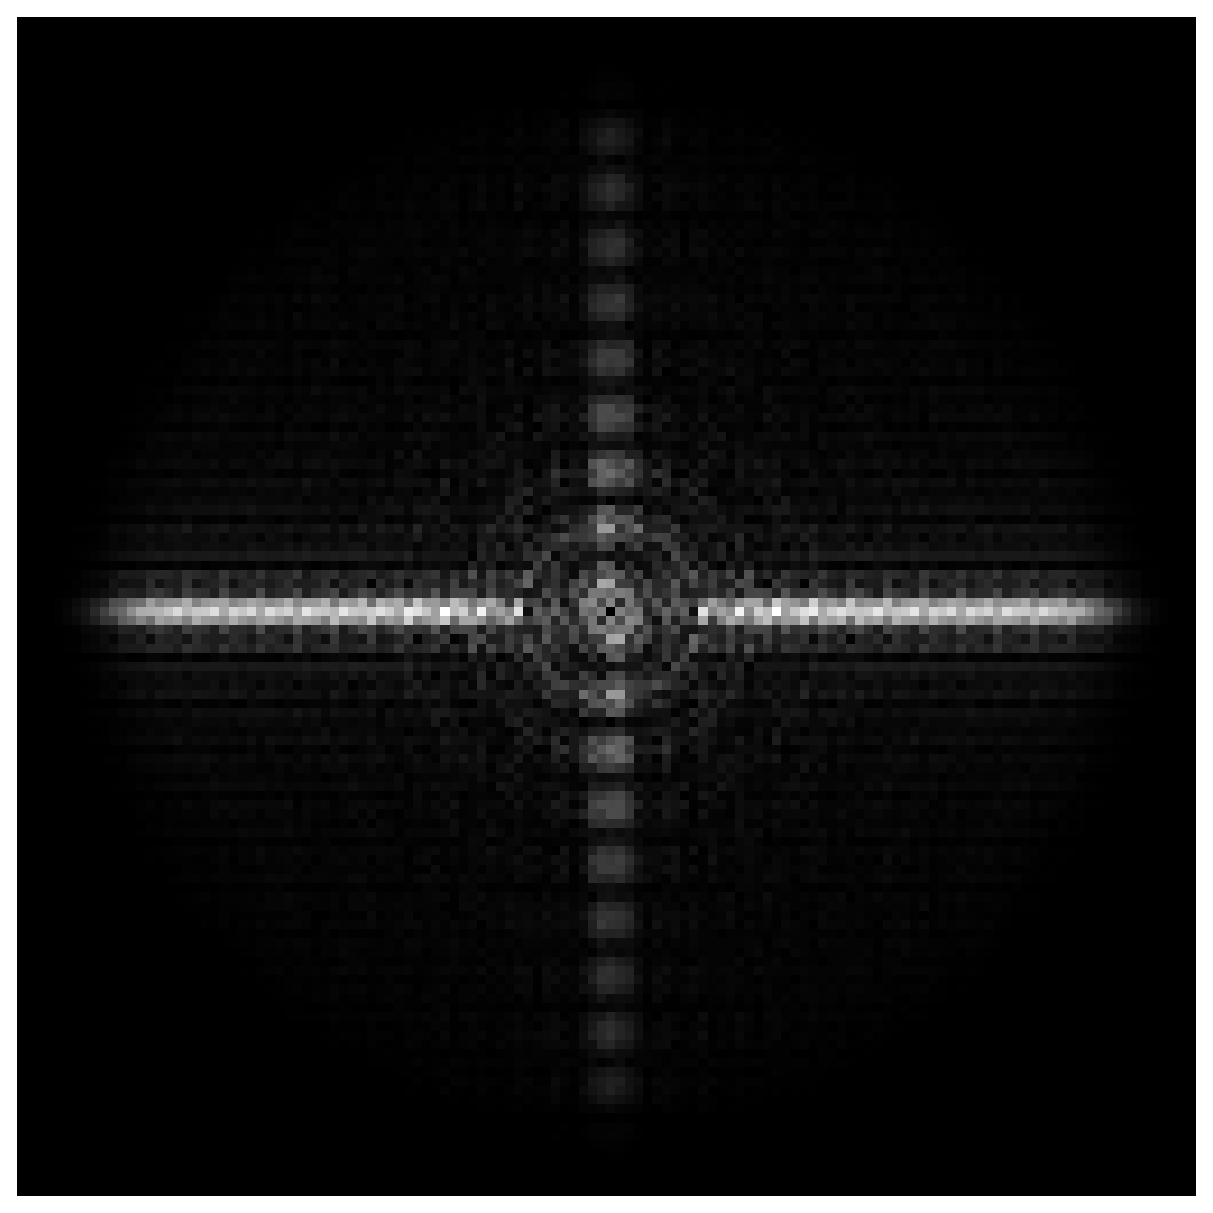
\includegraphics[width=4cm]{../app_hilo/kihp3}}
  \caption{The Fouriertransform of the shifted zero-order-suppressed
    non-uniform image $q_s$ with (a) and without (b) low-pass filter
    and the Fouriertransform of the corrected high-pass filtered
    uniform image (c). As opposed to all other k-space images (b) and
    (c) are not logarithmic.}
  \label{fig:hilo3_2}
\end{figure}

The following listing shows how the image is non-uniform image is
shifted in k-space so that the first order becomes dc. This result
$\hat q_s$ is shown in \figref{fig:kqs}.
\begin{lstlisting}
%% multiply by this in object space to shift +1 order into middle
doshift=exp(-i*2*pi*(xx(ckin,'freq').*shift(1)+yy(ckin,'freq').*shift(2)));
%%
kc=0.052;
r=rr(ckin,'freq');
klp=exp(-r.^2/(2*kc^2)); % low pass filter in k-space
q1=ift(ckin-kappa.*ckiu);
kqs=ft(q1.*doshift);
cm=abs(ift(kqs.*klp));
ihp=real(ift(ft(iu).*corr.*(1-klp)));
% integrate over ring with radius kc to find eta
ring=abs(ft(besselj(0,2*pi*kc*n.*r)));
ring2=r-1./n<kc & r+1./n>kc;
cring=ring.*ring2;
nring=cring./sum(abs(cring));
eta=sum(abs(ft(ihp))/abs(ft(cm)).*nring);
% combine highpass and lowpass filtered images
ihilo3=2.*cm+ihp; % don't use eta
\end{lstlisting}
The calculation of $\eta$ gives the value $1.16$. It turns out that
the reconstructed slice (\figref{fig:ihilo3}) looks better with a
value of $\eta=2$. This makes sense as the grating reduces the
illumination power by this factor. 
\begin{figure}[htb]
  \centering \subfigure[ {\tt
    cm}]{\label{fig:cm}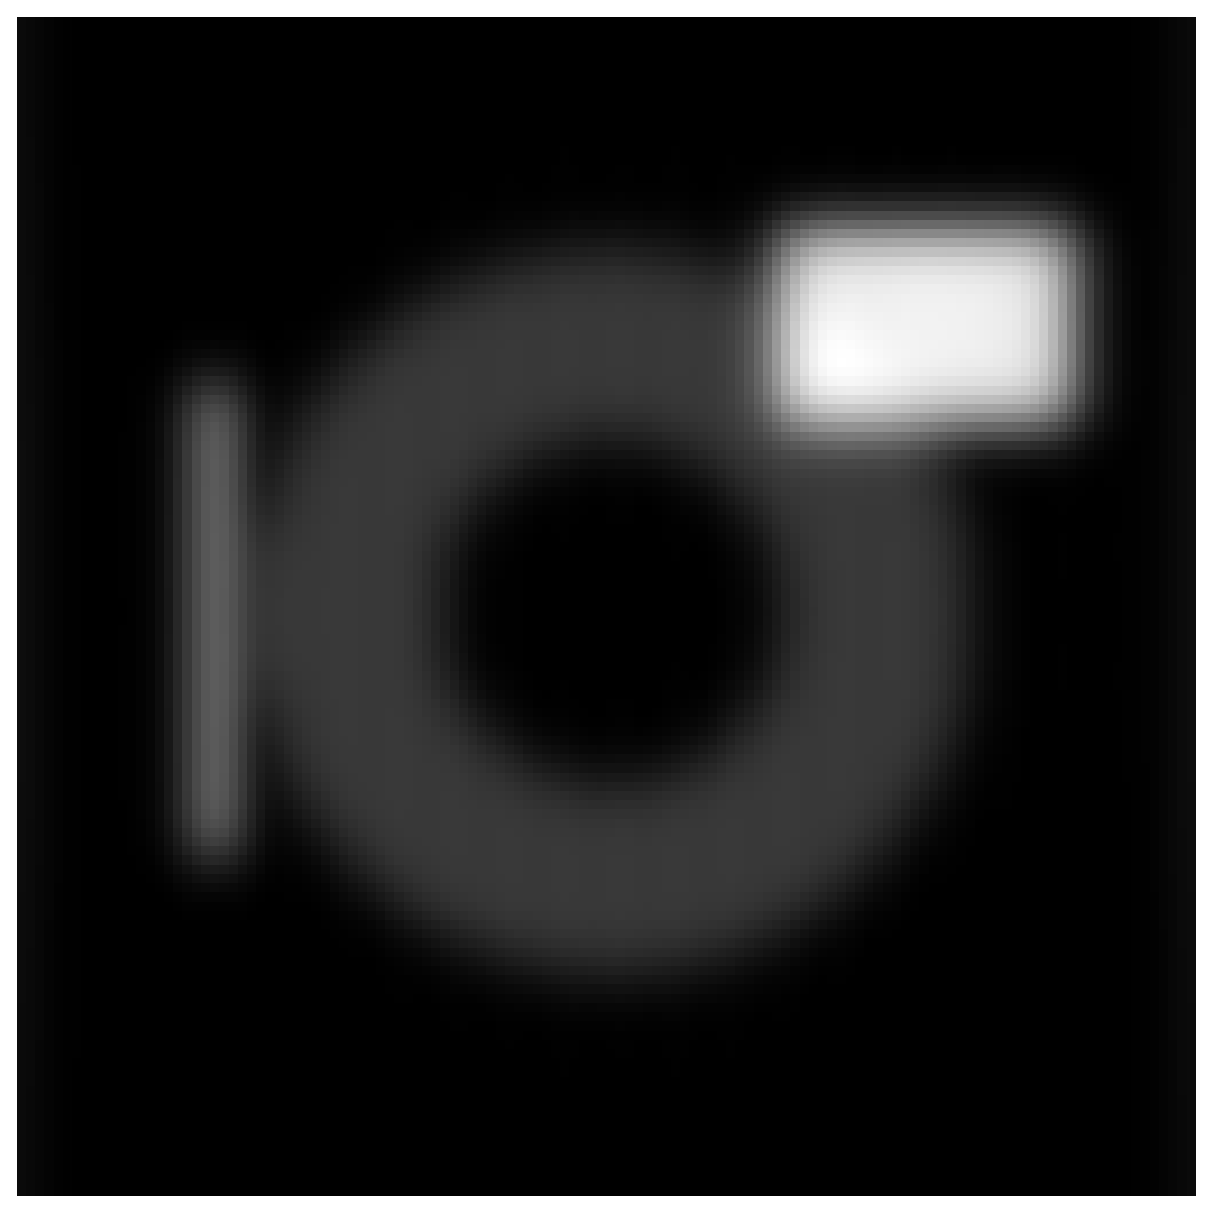
\includegraphics[width=4cm]{../app_hilo/cm}}
  \subfigure[$I_\textrm{hp}$]{\label{fig:ihp}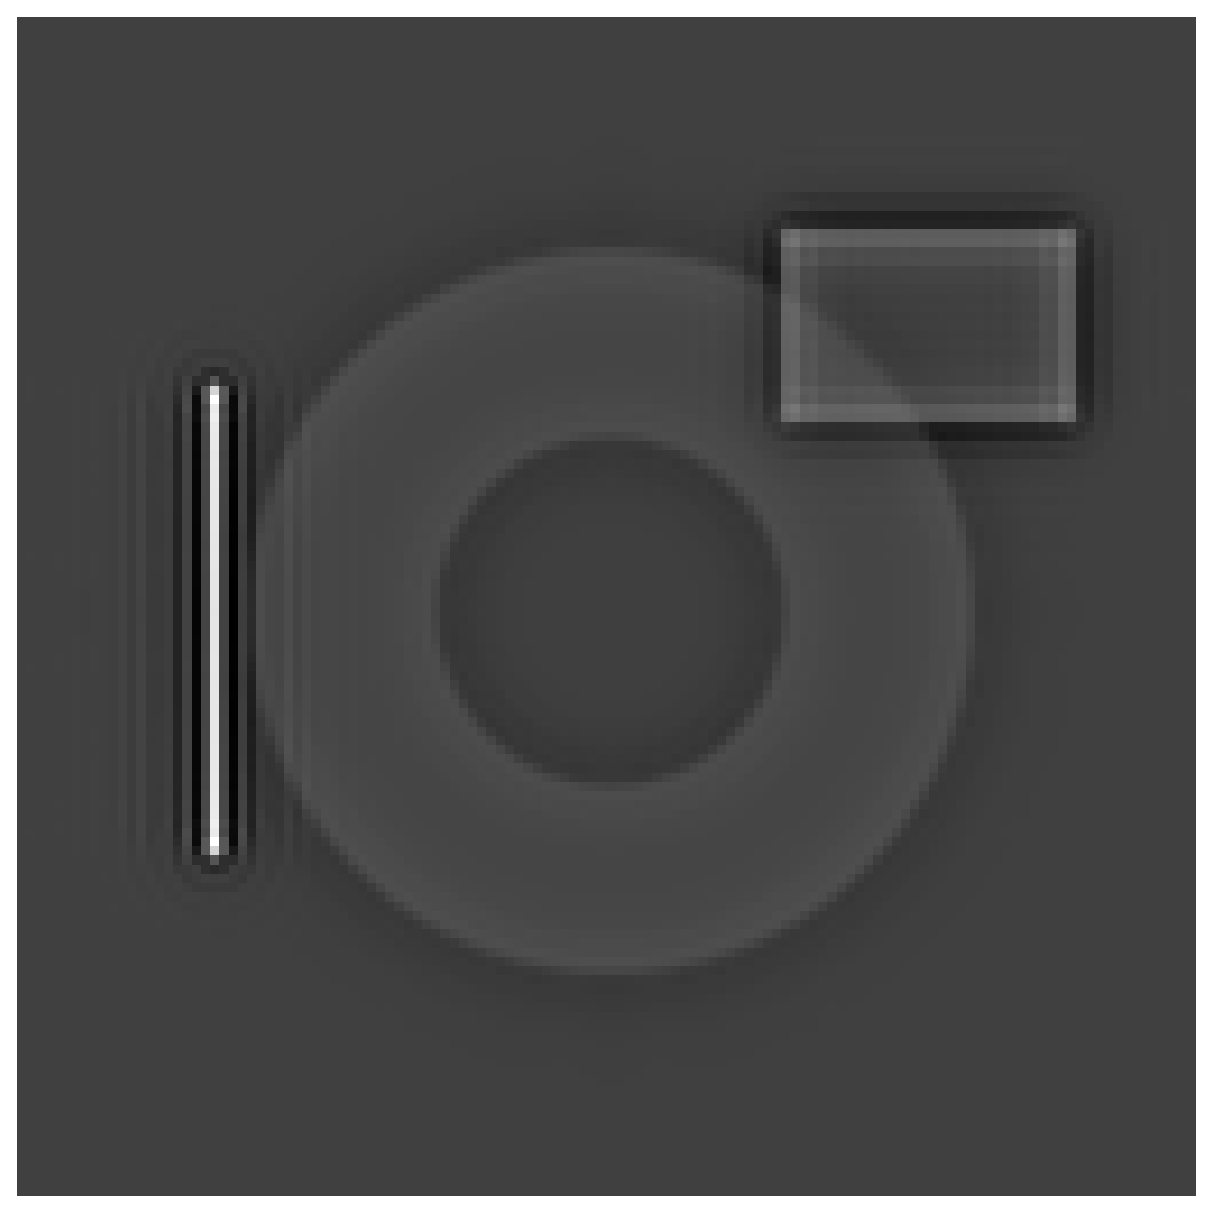
\includegraphics[width=4cm]{../app_hilo/ihp3}}
  \subfigure[$I_\textrm{hilo}$]{\label{fig:ihilo3}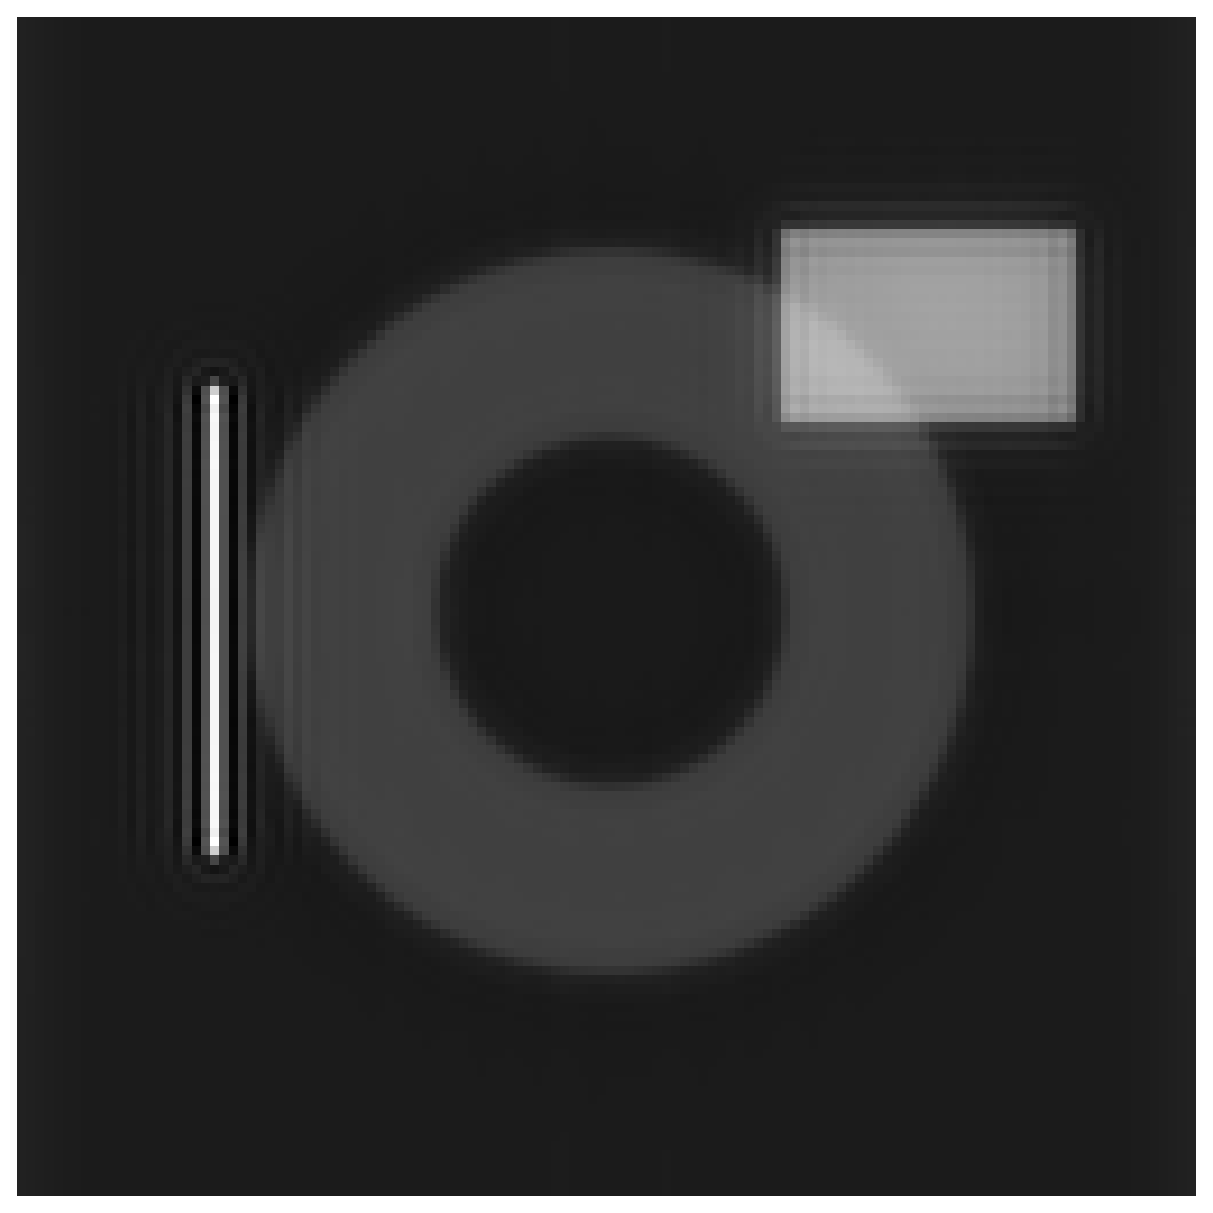
\includegraphics[width=4cm]{../app_hilo/ihilo3}}
  \caption{Low (a) and high-frequency (b) images in real space and the
    end result (c).}
  \label{fig:hilo3_3}
\end{figure}

\section{Acknowledgements}
I thank Rainer Heintzmann and Kai Wicker for fruitfull discussions
on k-space.

